\documentclass[dvipdfmx,a4paper,10pt]{article}
\usepackage[dvips]{graphicx}
\usepackage{subfigure}
\usepackage[small,bf]{caption}
\usepackage{color}
\usepackage{natbib,amsmath}
\usepackage[margin=2.5cm]{geometry}
\usepackage{hyperref}
\hypersetup{
  colorlinks = true,
  citecolor=red,%
  filecolor=red,%
  linkcolor=red,%
  urlcolor=red
  pdfsubject = {Report},
  pdfpagemode = UseNone
}

% Title Page
\title{Implementation of an EDMF boundary-layer and shallow-cumulus parameterization into CAMR}
\author{Wolfgang Langhans}


\begin{document}
\maketitle

\section{Introduction}\label{se:intro}

For any prognostic variable $\rho\psi$ we seek to represent its tendency due to unresolved turbulent transport. Thereby, $\psi$ is one of $u$, $v$, $\theta_v$, $q_v$, and eventually $e$ (i.e., TKE).\footnote{Turbulent kinetic energy $e$ is included here since -- depending on the applied eddy-diffusivity model -- a prognostic equation for $e$ has eventually to be solved.} Here, $q_v$ is defined as the mass of water vapor per mass of moist air, as $q_v=\rho_v/(\rho_d+\rho_v)$. It is common in GCMs and mesoscale models to assume that the vertical velocity $w$ has no tendency from subgrid-scale transport. On top of that, subgrid transport is assumed to be vertical only. 

The air density $\rho=\rho_d+\rho_v$ is affected by turbulent mixing since its moisture content changes. The updated values of $\rho$, $\rho_v$, and any other variable $\rho \psi$ are consistently obtained as 
\begin{eqnarray}
\rho^{n+1}&=&\rho^n + \Delta t \frac{\partial \rho}{\partial t}=\rho^n + \Delta t \frac{\partial \rho_v}{\partial t}=\rho^n + \Delta t \rho_d^n\left(\frac{\partial r_v}{\partial t}\right)_{turb} \\
\rho_v^{n+1}&=&\rho_v^n + \Delta t \rho_d^n\left(\frac{\partial r_v}{\partial t}\right)_{turb}\\
 (\rho\psi)^{n+1} &=& \rho^{n+1}\left[\psi^n + \Delta t \left(\frac{\partial \psi}{\partial t}\right)_{turb}\right]\\
\end{eqnarray}
whereby we used the fact that the density of dry air, $\rho_d=\frac{1-q_v}{q_v}\rho_v$, remains unchanged (i.e., we are only adding/removing water vapor molecules). Here $r_v=q_v/(1-q_v)$ is the mixing ratio of water vapor.  

The tendency for any variable $\psi$ (other than a mixing ratio) is then obtained from the EDMF equation as
\begin{equation}\label{eqn:tendency}
 \left(\frac{\partial \psi}{\partial t}\right)_{turb} =-\frac{1}{\rho}\frac{\partial }{\partial z} \rho \left( ED^{\psi} + MF^{\psi}\right) = -\frac{1}{\rho}\frac{\partial }{\partial z} \rho\left( -K_{\psi}(z)\frac{\partial \psi(z)}{\partial z} + \sum_i M_i(z) (\psi^{up}_i(z) - \psi(z) )\right)
\end{equation}
and the tendency for a mixing ratio (e.g., $r_v$) is analogously obtained with $\rho$ replaced by $\rho_d$. Here, ED is the eddy-diffusivity part and MF the (multiplume) mass-flux part of the turbulent flux. Closure is provided by specifying $K_{\psi}$, $M_i$, and $\psi^{up}_i$ for each updraft $i$.

The necessary/provided input to the EDMF parameterization is listed in section \ref{sec:input}. The closure is described in section \ref{sec:closure}. The numerical procedure to solve Eq. (\ref{eqn:tendency}) is outlined in section \ref{sec:solve}. One key advantage of this multiplume EDMF parameterization is that PBL mixing and shallow cumulus cloud cover are parameterized in a unified fashion since plumes might eventually get saturated. For this reason, several versions of EDMF also provide a subgrid-scale cloud cover (shallow cumulus and eventually also strato-cumulus) and unresolved cloud liquid water content which is then passed on to the radiative transfer code. The approach taken in this direction is described in section \ref{sec:clouds}.

\section{Input}\label{sec:input}

\subsection{From CAMR Dycore}

The prognostic variables $u$, $v$, $w$, $\theta_v$, $q_v$ and $\rho$ are provided at cell centers. In this 1D framework let index $k$ represent the vertical center of cell $k$. Let indices $k-1/2$ and $k+1/2$ indicate the position of the bottom and top interface of cell $k$. Thus, the input is $u^k$, $v^k$, $w^k$, $\theta_v^k$, $q_v^k$, and $\rho_k$ with $k$ ranging from $1$ to the total number of cells $N_k$ in the 1D column. On top of that, $\rho^{k\pm 1/2}$ will be needed from the Dycore. 

Also needed for the parameterization of eddy diffusivities is the squared characteristic rate of strain $\overline{D}^2$ (based on grid-scale velocities) as defined in Eq.~(\ref{eqn:def2}) at cell centers. 

\subsection{From surface flux parameterization}\label{sec:sfcfluxes}

The parameterization of surface fluxes over ocean surface is based on \cite{bryan03} and has been used also in SAM \citep{khairou03} and CAM \citep[see][section 4.10.2]{collins04}. A formulation for fluxes over land is also available but not yet included. The formulation is adapted here to our needs as explained below. A bulk drag/transfer law is used for the surface turbulent fluxes of $u$, $v$, $\theta$, and $r_v$, given as
\begin{equation}\label{eqn:fluxes}
 (\mathbf{\tau}, E, H)=-\rho_1|\mathbf{v_h}_1| (C_d \mathbf{v_h}_1, C_e \Delta r_v, C_{\theta} \Delta \theta )
\end{equation}
with $\Delta r_v=r_{v1}-r_v^*(T_s)$, $\Delta \theta=\theta_{1}-\theta_{s}$, $\mathbf{v_h}$ the horizontal wind vector, and $C_d$, $C_e$, and $C_{\theta}$ the transfer coefficients for momentum, $r_v$, and $\theta$. $T_s$ is the surface temperature and $r_v^*(T_s)$ the saturation mixing ratio at the surface temperature. Index ``$1$'' indicates values on the first model level. 

Turbulent velocity scales $u_*$, $r_{v*}$, and $\theta_{*}$ are introduced in the formulation of these fluxes as 
\begin{eqnarray}
 u_*&=& (\overline{u'w'}^2+\overline{v'w'}^2)^{1/4} = C_d^{1/2} | \mathbf{v_h}_1 |\\
 r_{v*}&=& -\overline{r_v'w'}/u_*=C_e |\mathbf{v_h}_1| \Delta r_v / u_*\label{eqn:velqv}
\end{eqnarray}

The parameterization characterizes the surface layer stability based on the Monin-Obukhov length and then distinguishes between flux profiles for stable and unstable conditions. The parameterization proceeds by utilizing similarity theory to determine the drag coefficients $C_d$, $C_e$, and $C_{\theta}$ and the respective fluxes. That is, the parameterization provides the sensible heat flux.  Note that here we seek a flux of $\theta_v$. The required flux in kinematic units is obtained as 
\begin{equation}\label{eqn:wthetav}
 \overline{\theta_v'w'}\approx \overline{\theta'w'}(1+0.61q_{v1}) + 0.61 \theta_1  \overline{r_v'w'}.
\end{equation}
This approximation implied dropping the contribution from the triple-correlation $\overline{w'q_v'\theta'}$ \citep[same as in Eq.~(10) in][]{stull94}. However, note that the flux of virtual potential temperature is commonly even further approximated as $\overline{\theta_v'w'}=\overline{\theta'w'}+0.61 \theta_1  \overline{r_v'w'}$ \citep[e.g.,][Eq.~(10.11)]{wyngaard10}. 

Using the bulk transfer law $H_v=-\rho_1|\mathbf{v_h}_1| C_{\theta_v}\Delta \theta_{v}$ and setting this equal to the flux obtained through (\ref{eqn:wthetav}) yields 
\begin{equation}\label{eqn:dragvirtual}
C_{\theta_v}=(C_h\Delta \theta [1+0.61q_{v1}] + 0.61 C_e\theta_1\Delta r_v)/ \Delta \theta_{v}. 
\end{equation}



\section{EDMF closure}\label{sec:closure}

The task of the parameterization is to provide the eddy diffusivities $K_{\psi}$ and $M_i$ and $\psi^{up}_i$ for each updraft $i$. A variety of flavors of the 1.5 TKE closure are implemented and described below. The updraft properties are obtained through a multiplume model that was kindly provided by Kay Suselj/JPL and somewhat modified here.


\subsection{Eddy-diffusivity models}

The eddy diffusivities are computed at cell centers and averaging provides $K_{\psi}^{k\pm 1/2}$ at cell interfaces. 

% \subsubsection{Smagorinsky closure}
% 
% This LES closure relates the eddy diffusivity for momentum to the characteristic rate of strain $\overline{D}$, as
% \begin{equation}\label{eqn:viscosity}
% K_m=(c_s l)^2 \overline{D}\sqrt{\max\left(0,1-\frac{\mathrm{Ri}}{\mathrm{Ri}_{c}}\right)}
% \end{equation}
% with the Richardson number defined as 
% \begin{equation}
%  \mathrm{Ri}=\left\{
% \begin{array}{ll}
% N_m^2/\overline{D}^2&\mathrm{for~saturated~air}\\
% N^2/\overline{D}^2&\mathrm{for~unsaturated~air}.
% \end{array}
% \right.  
% \end{equation} 
% and $\mathrm{Ri}_c=1.0$ a critical Richardson number and $N$ and $N_m$ the Brunt-V\"{a}is\"{a}l\"{a} frequencies in unsaturated and saturated air, respectively. Air is defined saturated if the mixing ratio of non-precipitating condensate is larger than a certain threshold. Equation (\ref{eqn:viscosity}) can be rewritten as 
% \begin{equation}
% K_m=(c_s l)^2 \sqrt{\max\left(0,\overline{D}^2-\frac{N^2}{\mathrm{Ri}_{c}}\right)}
% \end{equation}
% and equivalently using $N_m^2$ in case of saturated air (only $N^2$ is used for brevity below). The mixing length scale $l$ is stability dependent and expressed as
% \begin{equation}\label{eqn:lmixsmag}
%  l=\left\{ 
%  \begin{array}{ll}
%  \min(\Delta z, \max(0.1\Delta z, 0.76 \sqrt{(e/N^2)}))&\quad \mathrm{if}\quad N^2>0\\
%  \Delta z &\quad \mathrm{if}\quad N^2\leq 0.
%  \end{array}
% \right.  
% \end{equation}
% with $e$ the TKE distribution from the previous timestep that (ideally) got advected by the Dycore. TKE is then diagnosed as 
% \begin{equation}
%  e = (K_m/(c_kl))^2.
% \end{equation}
% The constant $c_s$ is given through the relation $c_s^4=c_k^3/c_e$ with $c_k=0.1$ and $c_e=0.54+1.44 l/\Delta z$. The eddy diffusivity for scalar transport is obtained as $K_h=\mathrm{Pr}K_m$ with the Prandtl number set to $\mathrm{Pr}=1/\mathrm{Ri}_c=1$. 
% 
% The square of the characteristic rate of strain $\overline{D}^2$ is defined as $\overline{D}^2=2D_{ij}D_{ij}$ with element $(i,j)$ of the tensor given as
% \begin{equation}
%  D_{ij}=\frac{1}{2}(\frac{\partial U_i}{\partial x_j}+\frac{\partial U_j}{\partial x_i})
% \end{equation}
% with capital $U$ indicating the grid-scale velocity and indices $i$ and $j$ are one of the three coordinate directions. After summation one obtains 
% \begin{equation}\label{eqn:def2}
%  \overline{D}^2=2\{D_{11}^2+D_{22}^2+D_{33}^2\}+4\{D_{12}^2+D_{13}^2+D_{23}^2 \}
% \end{equation}
% which is provided from the Dycore at cell centers. 


\subsubsection{Teixeira TKE closure}
The formulation of the TKE boundary layer scheme follows the description given by \cite{teixeira04} and is specifically designed here to model the evolution of the dry convective boundary layer. The prognostic equation for $e$, the sgs kinetic energy per unit dry air, is
\begin{eqnarray}\label{eqn:tkebudget}
 \frac{\partial e}{\partial t}&=& \mathrm{ADV} + \mathrm{TRANS} + \mathrm{SHEAR} + \mathrm{BUOY} - \mathrm{DISS}
\end{eqnarray}
and in this parameterization the individual sources/sinks are closed as
\begin{eqnarray}
 \mathrm{TRANS} &=& \frac{1}{\rho_d}\frac{\partial}{\partial z} (\rho_d K_m  \frac{\partial e}{\partial z})\\
 \mathrm{SHEAR} &=& K_m \overline{D}^2 \\
 \mathrm{BUOY} &=& \frac{g}{\theta_v}\overline{w'\theta_v'}\\
 \mathrm{DISS}&=& c_{\epsilon}\sqrt{e}/l_{\epsilon}
\end{eqnarray}
with $K_m=c_k l e^{1/2}$, $l_{\epsilon}=l/2.5$, $c_{\epsilon}=0.16$, and $c_k=0.5$. The square of the characteristic rate of strain $\overline{D}^2$ is defined as $\overline{D}^2=2D_{ij}D_{ij}$ with element $(i,j)$ of the tensor given as
\begin{equation}
 D_{ij}=\frac{1}{2}(\frac{\partial U_i}{\partial x_j}+\frac{\partial U_j}{\partial x_i})
\end{equation}
with capital $U$ indicating the grid-scale velocity and indices $i$ and $j$ are one of the three coordinate directions. After summation one obtains 
\begin{equation}\label{eqn:def2}
 \overline{D}^2=2\{D_{11}^2+D_{22}^2+D_{33}^2\}+4\{D_{12}^2+D_{13}^2+D_{23}^2 \}
\end{equation}
which is provided from the Dycore at cell centers. In the 1D case this reduces to $\overline{D}^2=(\frac{dU}{dz})^2+(\frac{dV}{dz})^2$.

The eddy diffusivity for heat and moisture fluxes is $K_h=\mathrm{Pr} K_m$ with $\mathrm{Pr}=1$. The mixing length is obtained as
\begin{eqnarray}
 l &=& \tau \sqrt{e} + (\kappa z - \tau \sqrt{e}) e^{-z/\alpha}
\end{eqnarray}
with $\alpha=100\mathrm{~m}$ and $\tau$ taken to be either 600 sec or $\tau=0.5 h/w^*$ with $w^*=(hg/\theta_{v0} \overline{w'\theta_v'}|_0)^{1/3}$. 
% The boundary layer height $h$ is defined as the level where the buoyancy flux is minimized. 
The TRANS diffusion term is solved in the same way as for any other scalar. The advective term ADV is eventually computed by the Dycore which has TKE per mass of moist air as prognostic variable such that conversion is required (i.e., analogous to the water vapor mixing ratio). 

The numerical implementation to advance $e$ from step $n$ to step $n+1$ is as follows. SHEAR, BUOY, and DISS are treated explicitly with an Euler step. Thereby, $K_m$ at step $n$ is diagnosed from $e$ at step $n$. In case the boundary layer height $h$ (defined as the level where the buoyancy flux is minimized) and $w^*$ are needed to evaluate mixing length $l$, the required buoyancy flux is obtained from the implicit computation for the previous time step. The three tendencies will be limited in magnitude to ensure their sum is not smaller than $-\frac{e}{\Delta t}$. Then, TRANS is computed as described below (general formulation allowing for an implicit solver) again based on the $e$ distribution (and $K$) at step $n$. That means that TRANS may still cause some negative $e$ at step $n+1$ since the solver for TRANS is not necessarily positive definite. Negative $e$ will be clipped at the beginning of the next step.

\subsubsection{Witek TKE closure}

\subsubsection{Langhans TKE closure}

\subsection{Multiplume model}

\subsubsection{Description}

The multiplume model provides updarft properties for a user-set number of plumes and thus the MF-part in Eq.~(\ref{eqn:tendency}). It closely follows the proposed multiplume model of \cite{cheinet03a}. Each plume represents one class of updrafts with the same thermodyniamic and kinematic properties. Note that in Eq.~(\ref{eqn:tendency}) it has been assumed that $\psi_d$ of the undisturbed subsiding air in the environment equals the grid-box mean $\psi$. This is equivalent to assuming that the updraft/downdraft area is small. This assumption is not made in, e.g., \cite{cheinet03a}. Following \cite{suselj12}, \cite{suselj13}, and \cite{suselj14} the MF part is assumed to be zero in case of $\psi$ equal to $u$, $v$, or $e$. This is generally justified by the smaller eddy viscosities for momentum than for heat and the general lack in knowledge about sources/sinks of momentum within a rising plume \citep[see, e.g., discussion in][]{han15}. Index $i$ identifies an individual updraft class among a total of $N^{up}$ (to be specified, e.g., $N^{up}=10$) updrafts. $M_i$ is defined as $s_i w^{up}_i$ with $s_i$ and $w^{up}_i$ the fractional weight and vertical velocity, respectively, of updraft class $i$. 


Initial conditions are obtained as in \cite{cheinet03a} and \cite{lenschow80}. Through similarity theory the initial conditions are linked to surface fluxes, boundary layer depth, and an assumed PDF of the vertical velocity. The latter is assumed to be a Gaussian with standard deviation $\sigma_w$, given as

\begin{equation}
 f_w(w) = \frac{1}{\sigma_w 2 \pi } e^{-\frac{w^2}{2\sigma_w^2}}.
\end{equation}


A fixed number of plumes spans a discrete PDF for a selected range between $w_{\mathrm{min}}$ and $w_{\mathrm{max}}$. Plume $i$ covers all vertical velocities between

\begin{eqnarray}
 w_i^{\mathrm{min}}&=&w_{\mathrm{min}}+(i-1)(w_{\mathrm{max}}-w_{\mathrm{min}})/N^{up} \qquad\mathrm{and}\\
 w_i^{\mathrm{max}}&=&w_{\mathrm{min}}+i(w_{\mathrm{max}}-w_{\mathrm{min}})/N^{up},
\end{eqnarray}
has a fractional weight  
\begin{equation}
 s_i =1/2(\mathrm{erf}(\frac{w_i^{\mathrm{max}}}{\sqrt{2}\sigma_w}) - \mathrm{erf}(\frac{w_i^{\mathrm{min}}}{\sqrt{2}\sigma_w})),
\end{equation}
and an average initial updraft velocity of 
\begin{equation}
 w_i =   \frac{\sigma_w}{s_i \sqrt{2 \pi }} (e^{-\frac{{w_i^{\mathrm{min}}}^2}{2 \sigma_w^2}}- e^{-\frac{{w_i^{\mathrm{max}}}^2}{2 \sigma_w^2}}).
\end{equation}
This initial average velocity has been modified here from the original $1/2(w_i^{\mathrm{min}}+w_i^{\mathrm{max}})$ used by Kay/JPL in order to make sure that the total upward mass flux $\rho \int\limits_0^{\infty} dw~f_w w = \rho \int\limits_0^{\infty} ds~ w=\rho \sum_{i=1,N_p} s_i w_i $ is independent of $N_p$. To illustrate the difference, if $w_{\mathrm{min}}=0$ and $w_{\mathrm{max}}\gg\sqrt{2}\sigma_w$ then the total area covered by updrafts is 0.5. Then, if only one plume was used, the average initial velocity would be $w_1=\sqrt{\frac{2}{\pi}} \sigma_w$ and not $0.5 w_i^{\mathrm{max}}$ as in the unmodified code. This update should allow for better convergence characteristics with an increasing number of plumes. 


The actual physical area fraction $f_i$ of a class spanned between $w_i^{\mathrm{min}}$ and $w_i^{\mathrm{max}}$ results from 
$\int\limits_{w_i^{\mathrm{min}}}^{w_i^{\mathrm{max}}} dw~ f(w) =\frac{1}{A_{tot}}\int\limits dA~N^*_i a_i$ with $N^*_i$ the number density (m$^{-2}$) and $a_i$ the areal extent of updrafts with velocities in the range $w_i^{\mathrm{min}}<w<w_i^{\mathrm{max}}$. The distributions $N^*_i(x,y)$ and $a_i(x,y)$ are defined to be zero whenever $w(x,y)$ falls outside of the specified range of the class. Of course, we can try and assume that all updrafts in one class have the same size such that 

\begin{equation}
 f_i = \frac{\int\limits_{w_i^{\mathrm{min}}}^{w_i^{\mathrm{max}}} dw~ f(w) }{ \int\limits_{A_{tot}} dA~N^*_i}= \frac{s_i }{ N_i}.
\end{equation}

Specifying $s_i$ thus leaves us to specify either the total number of updrafts represented by class $i$ or their fractional area $f_i$, but obviously not both.

Initial thermodynamic properties are obtained through similarity relations, as 
\begin{eqnarray}
 q_{vi}&=&q_{v}+0.32 w_i  \sigma_{q_t}/\sigma_w\\
 \theta_{vi}&=&\theta_{v}+0.58 w_i  \sigma_{\theta_v}/\sigma_w\\
  \theta_{li}&=&\theta_{vi}/(1+\epsilon q_{vi})=\theta_i \quad\mathrm{since}~q_{li}=0\\
  w^*&=&(hg/\theta_v \overline{w'\theta_v'})^{1/3}\\
  q_v^*&=&\overline{w'q_v'}/w^*\\
  \theta_v^*&=&\overline{w'\theta_v'}/w^*\\
 \sigma_w&=&1.34 w^*(z_s/h)^{1/3} (1-0.8z_s/h)\\
   \sigma_{q_t}&=&1.34 q_v^* (z_s/h)^{-1/3}\\
  \sigma_{\theta_v}&=&1.34\theta_v^* (z_s/h)^{-1/3}
\end{eqnarray}
with coefficients chosen in agreement with \cite{lenschow80} and the boundary layer height $h$ defined as the level where the buoyancy flux gets minimized. $z_s$ is set to be 50 meter and supposed to be in the surface layer. 

Steady-state plumes are used to describe the vertical profile of the properties in entraining and ascending parcels. A conserved quantity $\psi$ follows the vertical profile given by
\begin{eqnarray}\label{eqn:conserved}
 \frac{d\psi_i^{up} }{d z } &=& - \epsilon(\psi_i^{up} - \psi)
\end{eqnarray}
with entrainment rate $\epsilon$ and the environmental value $\psi$. The parcel rises until its vertical velocity reaches zero. The latter is given by
\begin{eqnarray}\label{eqn:w}
 \frac{d (w_i^{up})^2 }{d z } &=& 2aB^{up}_i- (2b+c\epsilon)(w_i^{up})^2
\end{eqnarray}
with buoyancy $B_i^{up}=g(\theta_v^{up}/\theta_v-1)$, the environmental profile $\theta_v$, and constants $a$, $b$, and $c$. The three acceleration terms are buoyancy, form drag, and mixing drag. 


The conserved variables used in the plume equations are liquid water potential temperature $\theta_l$ and total water mass fraction $q_t=q_v+q_l$. Equation (\ref{eqn:conserved}) is solved for these two variables until the vertical velocity in a plume turns zero. At each height a saturation adjustment scheme is used to infer the liquid water content $q_l$, $q_v$, and $\theta_v$. 


\subsubsection{Discretization}
Solving the vertical velocity and scalar equation in the vertical is accomplished as in \cite{suselj14} (see their appendix). Thereby we assume that $\epsilon$, the environment value $\psi$, and buoyancy $B$ can be considered constant in each layer (instead of, e.g., $\epsilon(\psi^{up}-\psi)$ being constant) to obtain an analytical expression for $\psi$ at the next level. This method has the numerical advantage that $\psi^{up}$ at the next higher level will be bound in between the value of $\psi^{up}$ at the lower level and the environmental value of $\psi$ in that layer. This provides the mass flux properties ($M_i^{k\pm 1/2}$ and $\psi^{up~k\pm 1/2}_i$) on cell interfaces. The discretized equations are 
\begin{eqnarray}
 \psi_i^{up~k+1/2}&=&\psi^{~k}(1-e^{-\epsilon^{k}\Delta z^k})+\psi_i^{up~k-1/2}e^{-\epsilon^{k}\Delta z^k}\\
 (w_i^{up~k+1/2})^2&=&(\alpha w_i^{up~k-1/2})^2 + (1-\alpha^2) \frac{aB_i^{up~k}}{b+c\epsilon^k},
\end{eqnarray}
where $\alpha=e^{-(b+c\epsilon^k)\Delta z^k}$ and $B_i^{up~k}=g(0.5(\theta_{vi}^{up~k+1/2}+\theta_{vi}^{up~k-1/2})/\theta_v^{k}-1)$. The entrainment rate (m$^{-1}$) in layer $\Delta z^k$ is computed as
\begin{equation}
 \epsilon(\Delta z^k) = \frac{1}{\Delta z^k} \epsilon_d \mathcal{P}(\frac{\Delta z^k}{L_0})
\end{equation}
with $\epsilon_d=0.1$, $L_0=100$~m, $a=2/3$, $b=0.002$~m$^{-1}$, $c=1.5$, and $\mathcal{P}$ a random number drawn from the Poisson distribution. The entrainment rate is thus so far formulated identically for the different updraft classes. 

\section{Solving for the tendency}\label{sec:solve}

Equation (\ref{eqn:tendency}) needs to be solved to obtain tentendy $T^{\psi}$. The spatial discretization of the equations is done using a centered scheme for the diffusion term and the mass-flux term. $K$, $M_i$, and $\psi^{up}_i$ are treated explicitly in time while other terms can be implicit. \footnote{If the prognostic TKE closure is used then SAM would use an intermediate $K$ obtained from an intermediate $e$ that got advanced through a truncated budget (\ref{eqn:tkebudget}) without the TRANS term. TRANS (i.e. mixing) is then computed based on the intermediate $e$ and $K$. We find, however, that this approach leads to strange instabilities in a CPBL test. Thus, we use a truly explicit approach for $e$ and $K$.} For brevity we drop index $_\psi$ here for eddy diffusivities $K$. The vertical grid structure and the indexing is illustrated in Fig.~\ref{fig:staggering} and is the same as used by \cite{tiedtke89}. An important stability criterion -- realized by \cite{tiedtke89} -- is that the environmental value of $\psi$ at the interface $k+1/2$ can not be taken as the average between $k$ and $k+1$. The interface value of $\psi$ is needed in the subsidence term $- \psi(z) \sum_i M_i(z)$ and in line with an upwind discretization has to be interpolated/taken from above. Since all prognostic variables are to a good approximation conserved along the unsaturated downdraft (besides detrainment effects) we simply say $\psi^{k+1/2}=\psi^{k+1}$ and  $\psi^{k-1/2}=\psi^{k}$. We find that taking the average indeed results in numerical instabilities, while this approach works fine. The discretized form of Eq. (\ref{eqn:tendency}) is then
\begin{align*}
  &\frac{\psi^{n+1,k}- \psi^{n,k} }{\Delta t} =\\
  &-\frac{1}{\rho^{n,k}\Delta z^{k}}\left\{ -\frac{K^{n,k+1/2}\rho^{n,k+1/2} }{\Delta z^{k+1/2}} [\beta_1^+(\psi^{n+1,k+1}-\psi^{n+1,k}) + \beta_1^-(\psi^{n,k+1}-\psi^{n,k})] \right. \\
    & \left.+\frac{K^{n,k-1/2}\rho^{n,k-1/2} }{\Delta z^{k-1/2}} [\beta_1^+(\psi^{n+1,k}-\psi^{n+1,k-1}) + \beta_1^-(\psi^{n,k}-\psi^{n,k-1})] \right.\\
    & \left. +\rho^{n,k+1/2}\left[\sum_i M_i^{n,k+1/2}\psi_i^{up~n,k+1/2} - (\beta_2^+\psi^{n+1,k+1}+\beta_2^-\psi^{n,k+1} )\sum_i M_i^{n,k+1/2} \right]\right.\\
    &\left.-\rho^{n,k-1/2}\left[\sum_i M_i^{n,k-1/2}\psi_i^{up~n,k-1/2} -(\beta_2^+\psi^{n+1,k}+\beta_2^-\psi^{n,k} )\sum_i M_i^{n,k-1/2} \right] \right\}\\
\end{align*}
with $\beta_1^+=1-\beta_1^-$ and $\beta_2^+=1-\beta_2^-$ the implicit weights. A fully implicit solver, i.e., $\beta_1^{+}=\beta_2^{+}=1$, is mostly used here. A tridiagonal matrix solver is used to solve $\mathbf{A}\cdot\Psi^{n+1}=\mathbf{d}$ for $\Psi^{n+1}$. 

\noindent For $2\leq k \leq N_k-1$ the coefficients are given as 

\begin{align*}
  a_k &=  \frac{\rho^{n,k-1/2}}{\rho^{n,k}\Delta z^k} \left[\beta_1^+ \frac{K^{n,k-1/2}}{\Delta z ^{k-1/2}}\right]\\
    b_k &= -\frac{1}{\Delta t} + \frac{\rho^{n,k+1/2}}{\rho^{n,k}\Delta z^k} \left[-\beta_1^+\frac{K^{n,k+1/2}}{\Delta z ^{k+1/2}} \right]-\frac{\rho^{n,k-1/2}}{\rho^{n,k}\Delta z^k} \left[\beta_1^+\frac{K^{n,k-1/2}}{\Delta z ^{k-1/2}}+\beta_2^+\sum_iM_i^{n,k-1/2} \right] \\
      c_k &= \frac{\rho^{n,k+1/2}}{\rho^{n,k}\Delta z^k}\left[\beta_1^+ \frac{K^{n,k+1/2}}{\Delta z ^{k+1/2}}+\beta_2^+\sum_iM_i^{n,k+1/2} \right] \\
      d_k &=-\frac{\psi^{n,k}}{\Delta t} - \frac{1}{\rho^{n,k}\Delta z^k} \left\{ \frac{K^{n,k+1/2}\rho^{n,k+1/2}}{\Delta z^{k+1/2}}\beta_1^{-}\left[\psi^{n,k+1} - \psi^{n,k}\right]-\frac{K^{n,k-1/2}\rho^{n,k-1/2}}{\Delta z^{k-1/2}}\beta_1^{-}\left[\psi^{n,k} - \psi^{n,k-1}\right]\right.   \\   
          & \left.+\rho^{n,k-1/2}\left[\sum_iM_i^{n,k-1/2}\psi_i^{up~n,k-1/2} - \beta_2^{-}\psi^{n,k}\sum_iM_i^{n,k-1/2} \right]\right.\\
          & \left. -\rho^{n,k+1/2}\left[\sum_iM_i^{n,k+1/2}\psi_i^{up~n,k+1/2} - \beta_2^{-}\psi^{n,k+1}\sum_iM_i^{n,k+1/2} \right] \right\}.
\end{align*}

\noindent The boundary conditions at the surface are specified for $k=1$, as

\begin{align*}
  a_k &= 0 \\
    b_k &= -\frac{1}{\Delta t} +\frac{\rho^{n,k+1/2}}{\rho^{n,k}\Delta z^k} \left[- \beta_1^+\frac{K^{n,k+1/2}}{\Delta z^{k+1/2}} \right]-\beta_1^+|\mathbf{v_{h1}}|C^n_{\psi}/\Delta z^k  \\
      c_k &= \mathrm{same~as~for~}2\leq k \leq N_k-1 \\
      d_k &=  -\frac{\psi^{n,k}}{\Delta t} - \frac{1}{\rho^{n,k}\Delta z^k} \left\{ \frac{K^{n,k+1/2}\rho^{n,k+1/2}}{\Delta z^{k+1/2}}\beta_1^{-}\left[\psi^{n,k+1} - \psi^{n,k}\right]\right.   \\   
          & \left. -\rho^{n,k+1/2}\left[\sum_iM_i^{n,k+1/2}\psi_i^{up~n,k+1/2} -\beta_2^{-}\psi^{n,k+1}\sum_iM_i^{n,k+1/2} \right] \right\} +|\mathbf{v_{h1}}|\frac{C^n_{\psi}}{\Delta z^k}\left[\beta^-\psi^{n,k} - \psi_s\right]    
\end{align*}
This formulation with Dirichlet boundary conditions makes use of the drag coefficients computed in the surface scheme and through (\ref{eqn:dragvirtual}). The user can, however, also decide to use a Neuman boundary condition ({\tt doneuman=.true.}) using the fluxes from the surface scheme and from (\ref{eqn:wthetav}). In this case, the last rhs term in $b_k$ is dropped and the last term in $d_k$ becomes $- \overline{\psi'w'}^n/\Delta z^k$ makeing the surface fluxes fully explicit. This explicit Neuman boundary condition is also used if surface fluxes are prescribed ({\tt sfc\_tau\_fxd} or {\tt sfc\_flx\_fxd} respectively). Same as in \cite{deardorff74}, the surface flux of $e$ is assumed to be zero and the explicit Neuman condition is always used. Zero tke fluxes at the surface are in line with findings presented by \cite{mcbean75} (see arguments given along with Eqn. (13)) and \cite{lenschow74} (see their Fig. 8). Or, as \cite{fuhrmann10} nicely put it:  ``\dots a zero-gradient condition for $k$ [here $e$] can be interpreted physically as specifying a zero flux of turbulent kinetic energy normal to a wall. This condition should in fact hold quite generally, as a wall (be it rough or smooth) is neither a direct source nor a sink of turbulent kinetic energy.''

The boundary condition at the top for $k=N_k$ is given as
\begin{align*}
  a_k &= \mathrm{same~as~for~}2\leq k \leq N_k-1  \\
    b_k &= -\frac{1}{\Delta t} - \frac{\rho^{n,k-1/2}}{\rho^{n,k}\Delta z^k} \left[\beta_1^+\frac{K^{n,k-1/2}}{\Delta z ^{k-1/2}}+\beta_2^+\sum_iM_i^{n,k-1/2} \right] \\
      c_k &= 0 \\
      d_k &= -\frac{\psi^{n,k}}{\Delta t} + \frac{1}{\rho^{n,k}\Delta z^k} \left\{ \frac{K^{n,k-1/2}\rho^{n,k-1/2}}{\Delta z^{k-1/2}}\beta_1^{-}\left[\psi^{n,k} - \psi^{n,k-1}\right]\right.   \\   
          & \left.-\rho^{n,k-1/2}\left[\sum_iM_i^{n,k-1/2}\psi_i^{up~n,k-1/2} -\beta_2^{-}\psi^{n,k}\sum_iM_i^{n,k-1/2} \right]\right\}.    
\end{align*}
Again, $\rho$ needs to be replaced by $\rho_d$ in case of $\psi=r_v$ or $\psi=e$. 


 

\begin{figure}[bthp]
\centering
 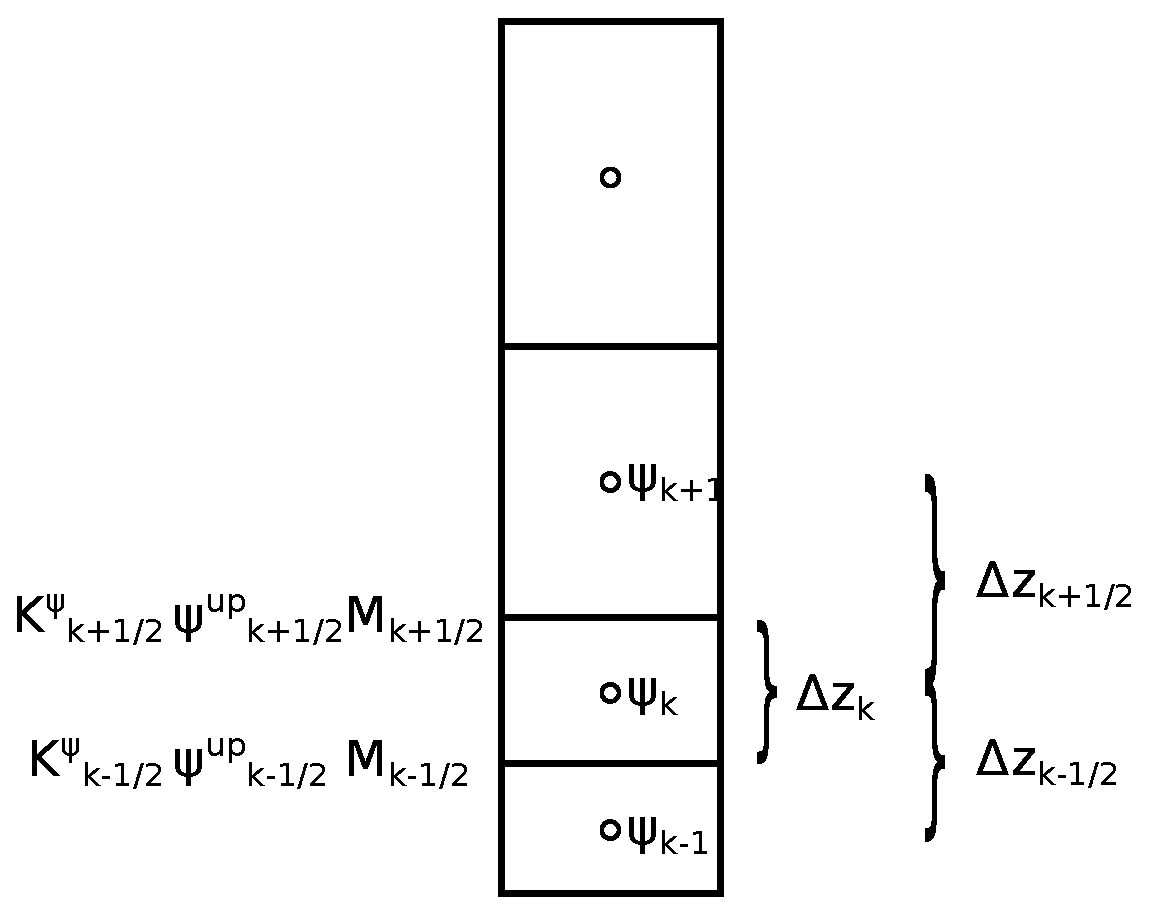
\includegraphics[width=0.5\textwidth]{staggering.eps}
\caption{Locations of prognostic variable $\psi$, the updraft mass fluxes $M_i$, the updraft properties $\psi^{up}_i$, and eddy-diffusivities $K^{\psi}$ on the 1D vertical grid. } \label{fig:staggering}
\end{figure}



\section{Cloud cover and interaction with radiation}\label{sec:clouds}

\subsection{Cumulus-topped PBL}

\subsection{Stratocumulus-topped PBL}



\section{Acknowledgements}
W.L. would like to thank Joao Teixeira and Kay Suselj for providing the code of their most recent version of the multiplume model. 


\bibliographystyle{ametsoc}
%\bibliography{/home/wolfi/Bibliography/wolfil_jab.bib}
\documentclass[dvipdfmx,a4paper,10pt]{article}
\usepackage[dvips]{graphicx}
\usepackage{subfigure}
\usepackage[small,bf]{caption}
\usepackage{color}
\usepackage{natbib,amsmath}
\usepackage[margin=2.5cm]{geometry}
\usepackage{hyperref}
\hypersetup{
  colorlinks = true,
  citecolor=red,%
  filecolor=red,%
  linkcolor=red,%
  urlcolor=red
  pdfsubject = {Report},
  pdfpagemode = UseNone
}

% Title Page
\title{Implementation of an EDMF boundary-layer and shallow-cumulus parameterization into CAMR}
\author{Wolfgang Langhans}


\begin{document}
\maketitle

\section{Introduction}\label{se:intro}

For any prognostic variable $\rho\psi$ we seek to represent its tendency due to unresolved turbulent transport. Thereby, $\psi$ is one of $u$, $v$, $\theta_v$, $q_v$, and eventually $e$ (i.e., TKE).\footnote{Turbulent kinetic energy $e$ is included here since -- depending on the applied eddy-diffusivity model -- a prognostic equation for $e$ has eventually to be solved.} Here, $q_v$ is defined as the mass of water vapor per mass of moist air, as $q_v=\rho_v/(\rho_d+\rho_v)$. It is common in GCMs and mesoscale models to assume that the vertical velocity $w$ has no tendency from subgrid-scale transport. On top of that, subgrid transport is assumed to be vertical only. 

The air density $\rho=\rho_d+\rho_v$ is affected from turbulent mixing since the moisture content changes. The updated values of $\rho$, $\rho_v$, and any other variable $\rho \psi$ are obtained as 
\begin{eqnarray}
\rho^{n+1}&=&\rho^n + \Delta t \frac{\partial \rho}{\partial t}=\rho^n + \Delta t \frac{\partial \rho_v}{\partial t}=\rho^n + \Delta t \rho_d^n\left(\frac{\partial r_v}{\partial t}\right)_{turb} \\
\rho_v^{n+1}&=&\rho_v^n + \Delta t \rho_d^n\left(\frac{\partial r_v}{\partial t}\right)_{turb}\\
 (\rho\psi)^{n+1} &=& \rho^{n+1}\left[\psi^n + \Delta t \left(\frac{\partial \psi}{\partial t}\right)_{turb}\right]\\
\end{eqnarray}
whereby we used the fact that the density of dry air $\rho_d=\frac{1-q_v}{q_v}\rho_v$ remains unchanged (i.e., we are only adding/removing water vapor molecules). Here $r_v=q_v/(1-q_v)$ is the mixing ratio of water vapor.  

The tendency for any variable $\psi$ (other than $r_v$) is then obtained from the EDMF equation as
\begin{equation}\label{eqn:tendency}
 \left(\frac{\partial \psi}{\partial t}\right)_{turb} =-\frac{1}{\rho}\frac{\partial }{\partial z} \rho \left( ED^{\psi} + MF^{\psi}\right) = -\frac{1}{\rho}\frac{\partial }{\partial z} \rho\left( -K_{\psi}(z)\frac{\partial \psi(z)}{\partial z} + \sum_i M_i(z) (\psi^{up}_i(z) - \psi(z) )\right)
\end{equation}
and the tendency for $r_v$ is analogously obtained with $\rho$ replaced by $\rho_d$. Here, ED is the eddy-diffusivity part and MF the mass-flux part of the turbulent flux. Closure is provided by specifying $K_{\psi}$ and $a_i$, $w^{up}_i$, and $\psi^{up}_i$ for each updraft $i$.

The necessary/provided input to the EDMF parameterization is listed in section \ref{sec:input}. The closure is described in section \ref{sec:closure}. The numerical procedure to solve Eq. (\ref{eqn:tendency}) is outlined in section \ref{sec:solve}. One key advantage of this multiplume EDMF parameterization is that PBL mixing and shallow cumulus cloud cover are parameterized in a unified fashion. For this reason, several versions of EDMF also provide a subgrid-scale cloud cover (cumulus and eventually strato-cumulus) and cloud liquid water content which is then passed on to the radiative transfer code. The approach taken in this implementation is described in section \ref{sec:clouds}.

\section{Input}\label{sec:input}

\subsection{From CAMR Dycore}

The prognostic variables $u$, $v$, $w$, $\theta_v$, $q_v$ and $\rho$ are provided at cell centers. In this 1D framework let index $k$ represent the vertical center of cell $k$. Let indices $k-1/2$ and $k+1/2$ indicate the position of the bottom and top interface of cell $k$. Thus, the input is $u^k$, $v^k$, $w^k$, $\theta_v^k$, $q_v^k$, and $\rho_k$ with $k$ ranging from $1$ to the total number of cells $N_k$ in the 1D column. On top of that, $\rho^{k\pm 1/2}$ will be needed from the Dycore. 

Also needed for the parameterization of eddy diffusivities is the squared characteristic rate of strain $\overline{D}^2$ (based on grid-scale velocities) as defined in Eq.~(\ref{eqn:def2}) at cell centers. 

\subsection{From surface flux parameterization}\label{sec:sfcfluxes}

The parameterization of surface fluxes over ocean surface is based on \cite{bryan03} and has been used also in SAM \citep{khairou03} and CAM \citep[see][section 4.10.2]{collins04}. A formulation for fluxes over land is also available but not yet included. The formulation is adapted here to our needs as explained below. A bulk drag/transfer law is used for the surface turbulent fluxes of $u$, $v$, $\theta$, and $r_v$, given as
\begin{equation}\label{eqn:fluxes}
 (\mathbf{\tau}, E, H)=-\rho_1|\mathbf{v_h}_1| (C_d \mathbf{v_h}_1, C_e \Delta r_v, C_{\theta} \Delta \theta )
\end{equation}
with $\Delta r_v=r_{v1}-r_v^*(T_s)$, $\Delta \theta=\theta_{1}-\theta_{s}$, $\mathbf{v_h}$ the horizontal wind vector, and $C_d$, $C_e$, and $C_{\theta}$ the transfer coefficients for momentum, $r_v$, and $\theta$. $T_s$ is the surface temperature and $r_v^*(T_s)$ the saturation mixing ratio at the surface temperature. Index ``$1$'' indicates values on the first model level. 

Turbulent velocity scales $u_*$, $r_{v*}$, and $\theta_{*}$ are introduced in the formulation of these fluxes as 
\begin{eqnarray}
 u_*&=& (\overline{u'w'}^2+\overline{v'w'}^2)^{1/4} = C_d^{1/2} | \mathbf{v_h}_1 |\\
 r_{v*}&=& -\overline{r_v'w'}/u_*=C_e |\mathbf{v_h}_1| \Delta r_v / u_*\label{eqn:velqv}
\end{eqnarray}

The parameterization characterizes the surface layer stability based on the Monin-Obukhov length and then distinguishes between flux profiles for stable and unstable conditions. The parameterization proceeds by utilizing similarity theory to determine the drag coefficients $C_d$, $C_e$, and $C_{\theta}$ and the respective fluxes. That is, the parameterization provides the sensible heat flux.  Note that here we seek a flux of $\theta_v$. The required flux in kinematic units is obtained as 
\begin{equation}\label{eqn:wthetav}
 \overline{\theta_v'w'}\approx \overline{\theta'w'}(1+0.61q_{v1}) + 0.61 \theta_1  \overline{r_v'w'}.
\end{equation}
This approximation implied dropping the contribution from the triple-correlation $\overline{w'q_v'\theta'}$ \citep[same as in Eq.~(10) in][]{stull94}. However, note that the flux of virtual potential temperature is commonly even further approximated as $\overline{\theta_v'w'}=\overline{\theta'w'}+0.61 \theta_1  \overline{r_v'w'}$ \citep[e.g.,][Eq.~(10.11)]{wyngaard10}. 

Using the bulk transfer law $H_v=-\rho_1|\mathbf{v_h}_1| C_{\theta_v}\Delta \theta_{v}$ and setting this equal to the flux obtained through (\ref{eqn:wthetav}) yields 
\begin{equation}\label{eqn:dragvirtual}
C_{\theta_v}=(C_h\Delta \theta [1+0.61q_{v1}] + 0.61 C_e\theta_1\Delta r_v)/ \Delta \theta_{v}. 
\end{equation}



\section{EDMF closure}\label{sec:closure}

The task of the parameterization is to provide the eddy diffusivities $K_{\psi}$ and $a_i$, $w^{up}_i$, and $\psi^{up}_i$ for each updraft $i$. For this implemetation, we decided to start by parameterizing the eddy diffusivities using 1-dimensional closures, either a Smagorinsky or a TKE closure. Both have been adapted and modified from SAM. The updraft properties are obtained through a multiplume model that was kindly provided by Kay Suselj/JPL.


\subsection{Eddy-diffusivity models}

Same as in SAM, the eddy diffusivities are computed at cell centers and averaging provides $K_{\psi}^{k\pm 1/2}$ at cell interfaces. 

\subsubsection{Smagorinsky closure}

This LES closure relates the eddy diffusivity for momentum to the characteristic rate of strain $\overline{D}$, as
\begin{equation}\label{eqn:viscosity}
K_m=(c_s l)^2 \overline{D}\sqrt{\max\left(0,1-\frac{\mathrm{Ri}}{\mathrm{Ri}_{c}}\right)}
\end{equation}
with the Richardson number defined as 
\begin{equation}
 \mathrm{Ri}=\left\{
\begin{array}{ll}
N_m^2/\overline{D}^2&\mathrm{for~saturated~air}\\
N^2/\overline{D}^2&\mathrm{for~unsaturated~air}.
\end{array}
\right.  
\end{equation} 
and $\mathrm{Ri}_c=1.0$ a critical Richardson number and $N$ and $N_m$ the Brunt-V\"{a}is\"{a}l\"{a} frequencies in unsaturated and saturated air, respectively. Air is defined saturated if the mixing ratio of non-precipitating condensate is larger than a certain threshold. Equation (\ref{eqn:viscosity}) can be rewritten as 
\begin{equation}
K_m=(c_s l)^2 \sqrt{\max\left(0,\overline{D}^2-\frac{N^2}{\mathrm{Ri}_{c}}\right)}
\end{equation}
and equivalently using $N_m^2$ in case of saturated air (only $N^2$ is used for brevity below). The mixing length scale $l$ is stability dependent and expressed as
\begin{equation}\label{eqn:lmixsmag}
 l=\left\{ 
 \begin{array}{ll}
 \min(\Delta z, \max(0.1\Delta z, 0.76 \sqrt{(e/N^2)}))&\quad \mathrm{if}\quad N^2>0\\
 \Delta z &\quad \mathrm{if}\quad N^2\leq 0.
 \end{array}
\right.  
\end{equation}
with $e$ the TKE distribution from the previous timestep that (ideally) got advected by the Dycore. TKE is diagnosed as $e = (K_m/(c_kl))^2$. The constant $c_s$ is given through the relation $c_s^4=c_k^3/c_e$ with $c_k=0.1$ and $c_e=0.54+1.44 l/\Delta z$. The eddy diffusivity for scalar transport is obtained as $K_h=\mathrm{Pr}K_m$ with the Prandtl number set to $\mathrm{Pr}=1/\mathrm{Ri}_c=1$. 

The square of the characteristic rate of strain $\overline{D}^2$ is defined as $\overline{D}^2=2D_{ij}D_{ij}$ with element $(i,j)$ of the tensor given as
\begin{equation}
 D_{ij}=\frac{1}{2}(\frac{\partial U_i}{\partial x_j}+\frac{\partial U_j}{\partial x_i})
\end{equation}
with capital $U$ indicating the grid-scale velocity and indices $i$ and $j$ are one of the three coordinate directions. After summation one obtains 
\begin{equation}\label{eqn:def2}
 \overline{D}^2=2\{D_{11}^2+D_{22}^2+D_{33}^2\}+4\{D_{12}^2+D_{13}^2+D_{23}^2 \}
\end{equation}
which is provided from the Dycore at cell centers. 


\subsubsection{TKE closure}
The formulation of the TKE boundary layer scheme follows the description given by \cite{teixeira04} and is specifically designed here to model the evolution of the convective boundary layer (and not as a LES closure). The prognostic equation for $e$, the sgs kinetic energy per unit dry air, is
\begin{eqnarray}\label{eqn:tkebudget}
 \frac{\partial e}{\partial t}&=& \mathrm{ADV} + \mathrm{TRANS} + \mathrm{SHEAR} + \mathrm{BUOY} - \mathrm{DISS}\\
 \mathrm{TRANS} &=& \frac{1}{\rho_d}\frac{\partial}{\partial z} (\rho_d K_m  \frac{\partial e}{\partial z})\\
 \mathrm{SHEAR} &=& K_m \overline{D}^2 \\
 \mathrm{BUOY} &=& \frac{g}{\theta_v}\overline{w'\theta_v'}\\
 \mathrm{DISS}&=& 0.16\cdot 2.5\sqrt{e}/l.
\end{eqnarray}
The virtual potential temperature flux is the sum of the ED and MF parts and computed at the end of the previous time step. The advective term is eventually computed by the Dycore which has TKE per mass of moist air as prognostic variable such that conversion is required (i.e., analogous to the water vapor mixing ratio). The eddy diffusivity for momentum is obtained as $K_m=0.5 l \sqrt{e}$ and $K_h=\mathrm{Pr} K_m$ with $\mathrm{Pr}=1$. The mixing length is obtained as
\begin{eqnarray}
 l &=& \tau \sqrt{e} + (\kappa z - \tau \sqrt{e}) e^{-z/\alpha}
\end{eqnarray}
with $\alpha=100\mathrm{~m}$ and $\tau$ taken to be either 600 sec or $\tau=h/w^*$ with $w^*=(hg/\theta_{v0} \overline{w'\theta_v'})^{1/3}$. The boundary layer height $h$ is defined as the level where the buoyancy flux is minimized. The TRANS diffusion term is solved in the same way as for any other scalar. Note that to obtain a standard LES TKE closure the mixing length can be defined same as in (\ref{eqn:lmixsmag}) and the coefficients in DISS can be adopted. 

The numerical implementation to advance $e$ from step $n$ to step $n+1$ is as follows. SHEAR, BUOY, and DISS are treated explicitly with an Euler step. Thereby, $K_m$ at step $n$ is diagnosed from $e$ at step $n$. In case the boundary layer height $h$ (defined as the level where the buoyancy flux is minimized) and $w^*$ are needed to evaluate mixing length $l$, the required buoyancy flux is obtained from the implicit computation for the previous time step. The three tendencies will be limited in magnitude to ensure their sum is not smaller than $-\frac{e}{\Delta t}$. Then, TRANS is computed as described below (general formulation allowing for an implicit solver) again based on the $e$ distribution at step $n$. That means that TRANS may still cause some negative $e$ at step $n+1$ since the solver for TRANS is not necessarily positive definite. Negative $e$ will be clipped at the beginning of the next step.   

\subsection{Multiplume model}

\subsubsection{Description}

The multiplume model provides updarft properties for a user-set number of plumes and thus the MF-part in Eq.~(\ref{eqn:tendency}). It closely follows the proposed multiplume model of \cite{cheinet03a}. Each plume represents one class of updrafts with the same thermodyniamic and kinematic properties. Note that in Eq.~(\ref{eqn:tendency}) it has been assumed that $\psi_d$ of the undisturbed subsiding air in the environment equals the grid-box mean $\psi$. This is equivalent to assuming that the updraft/downdraft area is small. This assumption is not made in, e.g., \cite{cheinet03a}. Following \cite{suselj12}, \cite{suselj13}, and \cite{suselj14} the MF part is assumed to be zero in case of $\psi$ equal to $u$, $v$, or $e$. This is generally justified by the smaller eddy viscosities for momentum than for heat and the general lack in knowledge about sources/sinks of momentum within a rising plume \citep[see, e.g., discussion in][]{han15}. Index $i$ identifies an individual updraft class among a total of $N^{up}$ (to be specified, e.g., $N^{up}=10$) updrafts. $M_i$ is defined as $s_i w^{up}_i$ with $s_i$ and $w^{up}_i$ the fractional weight and vertical velocity, respectively, of updraft class $i$. 


Initial conditions are obtained as in \cite{cheinet03a} and \cite{lenschow80}. Through similarity theory the initial conditions are linked to surface fluxes, boundary layer depth, and an assumed PDF of the vertical velocity. The latter is assumed to be a Gaussian with standard deviation $\sigma_w$, given as

\begin{equation}
 f_w(w) = \frac{1}{\sigma_w 2 \pi } e^{-\frac{w^2}{2\sigma_w^2}}.
\end{equation}


A fixed number of plumes spans a discrete PDF for a selected range between $w_{\mathrm{min}}$ and $w_{\mathrm{max}}$. Plume $i$ covers all vertical velocities between

\begin{eqnarray}
 w_i^{\mathrm{min}}&=&w_{\mathrm{min}}+(i-1)(w_{\mathrm{max}}-w_{\mathrm{min}})/N^{up} \qquad\mathrm{and}\\
 w_i^{\mathrm{max}}&=&w_{\mathrm{min}}+i(w_{\mathrm{max}}-w_{\mathrm{min}})/N^{up},
\end{eqnarray}
has a fractional weight  
\begin{equation}
 s_i =1/2(\mathrm{erf}(\frac{w_i^{\mathrm{max}}}{\sqrt{2}\sigma_w}) - \mathrm{erf}(\frac{w_i^{\mathrm{min}}}{\sqrt{2}\sigma_w})),
\end{equation}
and an average initial updraft velocity of 
\begin{equation}
 w_i =   \frac{\sigma_w}{s_i \sqrt{2 \pi }} (e^{-\frac{{w_i^{\mathrm{min}}}^2}{2 \sigma_w^2}}- e^{-\frac{{w_i^{\mathrm{max}}}^2}{2 \sigma_w^2}}).
\end{equation}
This initial average velocity has been modified here from the original $1/2(w_i^{\mathrm{min}}+w_i^{\mathrm{max}})$ used by Kay/JPL in order to make sure that the total upward mass flux $\rho \int\limits_0^{\infty} dw~f_w w = \rho \int\limits_0^{\infty} ds~ w=\rho \sum_{i=1,N_p} s_i w_i $ is independent of $N_p$. To illustrate the difference, if $w_{\mathrm{min}}=0$ and $w_{\mathrm{max}}\gg\sqrt{2}\sigma_w$ then the total area covered by updrafts is 0.5. Then, if only one plume was used, the average initial velocity would be $w_1=\sqrt{\frac{2}{\pi}} \sigma_w$ and not $0.5 w_i^{\mathrm{max}}$ as in the unmodified code. This update should allow for better convergence characteristics with an increasing number of plumes. 


The actual physical area fraction $f_i$ of a class spanned between $w_i^{\mathrm{min}}$ and $w_i^{\mathrm{max}}$ results from 
$\int\limits_{w_i^{\mathrm{min}}}^{w_i^{\mathrm{max}}} dw~ f(w) =\frac{1}{A_{tot}}\int\limits dA~N^*_i a_i$ with $N^*_i$ the number density (m$^{-2}$) and $a_i$ the areal extent of updrafts with velocities in the range $w_i^{\mathrm{min}}<w<w_i^{\mathrm{max}}$. The distributions $N^*_i(x,y)$ and $a_i(x,y)$ are defined to be zero whenever $w(x,y)$ falls outside of the specified range of the class. Of course, we can try and assume that all updrafts in one class have the same size such that 

\begin{equation}
 f_i = \frac{\int\limits_{w_i^{\mathrm{min}}}^{w_i^{\mathrm{max}}} dw~ f(w) }{ \int\limits_{A_{tot}} dA~N^*_i}= \frac{s_i }{ N_i}.
\end{equation}

Specifying $s_i$ thus leaves us to specify either the total number of updrafts represented by class $i$ or their fractional area $f_i$, but obviously not both.

Initial thermodynamic properties are obtained through similarity relations, as 
\begin{eqnarray}
 q_{vi}&=&q_{v}+0.32 w_i  \sigma_{q_t}/\sigma_w\\
 \theta_{vi}&=&\theta_{v}+0.58 w_i  \sigma_{\theta_v}/\sigma_w\\
  \theta_{li}&=&\theta_{vi}/(1+\epsilon q_{vi})=\theta_i \quad\mathrm{since}~q_{li}=0\\
  w^*&=&(hg/\theta_v \overline{w'\theta_v'})^{1/3}\\
  q_v^*&=&\overline{w'q_v'}/w^*\\
  \theta_v^*&=&\overline{w'\theta_v'}/w^*\\
 \sigma_w&=&1.34 w^*(z_s/h)^{1/3} (1-0.8z_s/h)\\
   \sigma_{q_t}&=&1.34 q_v^* (z_s/h)^{-1/3}\\
  \sigma_{\theta_v}&=&1.34\theta_v^* (z_s/h)^{-1/3}
\end{eqnarray}
with coefficients chosen in agreement with \cite{lenschow80} and the boundary layer height $h$ defined as the level where the buoyancy flux gets minimized. $z_s$ is set to be 50 meter and supposed to be in the surface layer. 

Steady-state plumes are used to describe the vertical profile of the properties in entraining and ascending parcels. A conserved quantity $\psi$ follows the vertical profile given by
\begin{eqnarray}\label{eqn:conserved}
 \frac{d\psi_i^{up} }{d z } &=& - \epsilon(\psi_i^{up} - \psi)
\end{eqnarray}
with entrainment rate $\epsilon$ and the environmental value $\psi$. The parcel rises until its vertical velocity reaches zero. The latter is given by
\begin{eqnarray}\label{eqn:w}
 \frac{d (w_i^{up})^2 }{d z } &=& 2aB^{up}_i- (2b+c\epsilon)(w_i^{up})^2
\end{eqnarray}
with buoyancy $B_i^{up}=g(\theta_v^{up}/\theta_v-1)$, the environmental profile $\theta_v$, and constants $a$, $b$, and $c$. The three acceleration terms are buoyancy, form drag, and mixing drag. 


The conserved variables used in the plume equations are liquid water potential temperature $\theta_l$ and total water mass fraction $q_t=q_v+q_l$. Equation (\ref{eqn:conserved}) is solved for these two variables until the vertical velocity in a plume turns zero. At each height a saturation adjustment scheme is used to infer the liquid water content $q_l$, $q_v$, and $\theta_v$. 


\subsubsection{Discretization}
Solving the vertical velocity and scalar equation in the vertical is accomplished as in \cite{suselj14} (see their appendix). Thereby we assume that $\epsilon$, the environment value $\psi$, and buoyancy $B$ can be considered constant in each layer (instead of, e.g., $\epsilon(\psi^{up}-\psi)$ being constant) to obtain an analytical expression for $\psi$ at the next level. This method has the numerical advantage that $\psi^{up}$ at the next higher level will be bound in between the value of $\psi^{up}$ at the lower level and the environmental value of $\psi$ in that layer. This provides the mass flux properties ($M_i^{k\pm 1/2}$ and $\psi^{up~k\pm 1/2}_i$) on cell interfaces. The discretized equations are 
\begin{eqnarray}
 \psi_i^{up~k+1/2}&=&\psi^{~k}(1-e^{-\epsilon^{k}\Delta z^k})+\psi_i^{up~k-1/2}e^{-\epsilon^{k}\Delta z^k}\\
 (w_i^{up~k+1/2})^2&=&(\alpha w_i^{up~k-1/2})^2 + (1-\alpha^2) \frac{aB_i^{up~k}}{b+c\epsilon^k},
\end{eqnarray}
where $\alpha=e^{-(b+c\epsilon^k)\Delta z^k}$ and $B_i^{up~k}=g(0.5(\theta_{vi}^{up~k+1/2}+\theta_{vi}^{up~k-1/2})/\theta_v^{k}-1)$. The entrainment rate (m$^{-1}$) in layer $\Delta z^k$ is computed as
\begin{equation}
 \epsilon(\Delta z^k) = \frac{1}{\Delta z^k} \epsilon_d \mathcal{P}(\frac{\Delta z^k}{L_0})
\end{equation}
with $\epsilon_d=0.1$, $L_0=100$~m, $a=2/3$, $b=0.002$~m$^{-1}$, $c=1.5$, and $\mathcal{P}$ a random number drawn from the Poisson distribution. The entrainment rate is thus so far formulated identically for the different updraft classes. 

\section{Solving for the tendency}\label{sec:solve}

Equation (\ref{eqn:tendency}) needs to be solved to obtain tentendy $T^{\psi}$. The spatial discretization of the equations is done using a centered scheme for the diffusion term and the mass-flux term. Same as in Teixeira and Siebesma (2000), \cite{siebesma07}, and \cite{soares04}, disretization in time is achieved using a fully implicit scheme for both the diffusion and the mass flux term. $K$, $M_i$, and $\psi^{up}_i$ are treated explicitly in time.\footnote{If the prognostic TKE closure is used then SAM would use an intermediate $K$ obtained from an intermediate $e$ that got advanced through a truncated budget (\ref{eqn:tkebudget}) without the TRANS term. TRANS (i.e. mixing) is then computed based on the intermediate $e$ and $K$. We find, however, that this approach leads to strange instabilities in a CPBL test. Thus, we use a truly explicit approach for $e$ and $K$.} See the discussion in \cite{siebesma07} (section 4c and appendix B) for further reference. For brevity we drop index $_\psi$ here for eddy diffusivities $K$. The vertical grid structure and the indexing is illustrated in Fig.~\ref{fig:staggering}. The discretized form of Eq. (\ref{eqn:tendency}) is
\begin{align*}
  &\frac{\psi^{n+1,k}- \psi^{n,k} }{\Delta t} =\\
  &-\frac{1}{\rho^{n,k}\Delta z^{k}}\left\{ -\frac{K^{n,k+1/2}\rho^{n,k+1/2} }{\Delta z^{k+1/2}} [\beta_1^+(\psi^{n+1,k+1}-\psi^{n+1,k}) + \beta_1^-(\psi^{n,k+1}-\psi^{n,k})] \right. \\
    & \left.+\frac{K^{n,k-1/2}\rho^{n,k-1/2} }{\Delta z^{k-1/2}} [\beta_1^+(\psi^{n+1,k}-\psi^{n+1,k-1}) + \beta_1^-(\psi^{n,k}-\psi^{n,k-1})] \right.\\
    & \left. +\rho^{n,k+1/2}\left[\sum_i M_i^{n,k+1/2}\psi_i^{up~n,k+1/2} - \frac{1}{2}(\beta_2^+\psi^{n+1,k}+\beta_2^-\psi^{n,k}+\beta_2^+\psi^{n+1,k+1}+\beta_2^-\psi^{n,k+1} )\sum_i M_i^{n,k+1/2} \right]\right.\\
    &\left.-\rho^{n,k-1/2}\left[\sum_i M_i^{n,k-1/2}\psi_i^{up~n,k-1/2} - \frac{1}{2}(\beta_2^+\psi^{n+1,k}+\beta_2^-\psi^{n,k}+\beta_2^+\psi^{n+1,k-1}+\beta_2^-\psi^{n,k-1} )\sum_i M_i^{n,k-1/2} \right] \right\}\\
\end{align*}
with $\beta_1^+=1-\beta_1^-$ and $\beta_2^+=1-\beta_2^-$ the implicit weights. A fully implicit solver, i.e., $\beta_1^{+}=\beta_2^{+}=1$, is used here to prevent instabilities. A tridiagonal matrix solver is used to solve $\mathbf{A}\cdot\Psi^{n+1}=\mathbf{d}$ for $\Psi^{n+1}$. 

\noindent For $2\leq k \leq N_k-1$ the coefficients are given as 

\begin{align*}
  a_k &=  \frac{\rho^{n,k-1/2}}{\rho^{n,k}\Delta z^k} \left[\beta_1^+ \frac{K^{n,k-1/2}}{\Delta z ^{k-1/2}}-\beta_2^+\frac{1}{2} \sum_iM_i^{n,k-1/2}\right]\\
    b_k &= -\frac{1}{\Delta t} + \frac{\rho^{n,k+1/2}}{\rho^{n,k}\Delta z^k} \left[-\beta_1^+\frac{K^{n,k+1/2}}{\Delta z ^{k+1/2}}+\beta_2^+\frac{1}{2}\sum_iM_i^{n,k+1/2} \right]-\frac{\rho^{n,k-1/2}}{\rho^{n,k}\Delta z^k} \left[\beta_1^+\frac{K^{n,k-1/2}}{\Delta z ^{k-1/2}}+\beta_2^+\frac{1}{2}\sum_iM_i^{n,k-1/2} \right] \\
      c_k &= \frac{\rho^{n,k+1/2}}{\rho^{n,k}\Delta z^k}\left[\beta_1^+ \frac{K^{n,k+1/2}}{\Delta z ^{k+1/2}}+\beta_2^+\frac{1}{2}\sum_iM_i^{n,k+1/2} \right] \\
      d_k &=-\frac{\psi^{n,k}}{\Delta t} - \frac{1}{\rho^{n,k}\Delta z^k} \left\{ \frac{K^{n,k+1/2}\rho^{n,k+1/2}}{\Delta z^{k+1/2}}\beta_1^{-}\left[\psi^{n,k+1} - \psi^{n,k}\right]-\frac{K^{n,k-1/2}\rho^{n,k-1/2}}{\Delta z^{k-1/2}}\beta_1^{-}\left[\psi^{n,k} - \psi^{n,k-1}\right]\right.   \\   
          & \left.+\rho^{n,k-1/2}\left[\sum_iM_i^{n,k-1/2}\psi_i^{up~n,k-1/2} - \frac{1}{2}\beta_2^{-}(\psi^{n,k}+\psi^{n,k-1})\sum_iM_i^{n,k-1/2} \right]\right.\\
          & \left. -\rho^{n,k+1/2}\left[\sum_iM_i^{n,k+1/2}\psi_i^{up~n,k+1/2} - \frac{1}{2}\beta_2^{-}(\psi^{n,k}+\psi^{n,k+1})\sum_iM_i^{n,k+1/2} \right] \right\}.
\end{align*}

\noindent The boundary conditions at the surface are specified for $k=1$, as

\begin{align*}
  a_k &= 0 \\
    b_k &= -\frac{1}{\Delta t} +\frac{\rho^{n,k+1/2}}{\rho^{n,k}\Delta z^k} \left[- \beta_1^+\frac{K^{n,k+1/2}}{\Delta z^{k+1/2}}+ \beta_2^+\frac{1}{2}\sum_iM_i^{n,k+1/2} \right]-\beta_1^+|\mathbf{v_{h1}}|C^n_{\psi}/\Delta z^k  \\
      c_k &= \mathrm{same~as~for~}2\leq k \leq N_k-1 \\
      d_k &=  -\frac{\psi^{n,k}}{\Delta t} - \frac{1}{\rho^{n,k}\Delta z^k} \left\{ \frac{K^{n,k+1/2}\rho^{n,k+1/2}}{\Delta z^{k+1/2}}\beta_1^{-}\left[\psi^{n,k+1} - \psi^{n,k}\right]\right.   \\   
          & \left. -\rho^{n,k+1/2}\left[\sum_iM_i^{n,k+1/2}\psi_i^{up~n,k+1/2} - \frac{1}{2}\beta_2^{-}(\psi^{n,k}+\psi^{n,k+1})\sum_iM_i^{n,k+1/2} \right] \right\} +|\mathbf{v_{h1}}|\frac{C^n_{\psi}}{\Delta z^k}\left[\beta^-\psi^{n,k} - \psi_s\right]    
\end{align*}
This formulation with Dirichlet boundary conditions makes use of the drag coefficients computed in the surface scheme and through (\ref{eqn:dragvirtual}). The user can, however, also decide to use a Neuman boundary condition ({\tt doneuman=.true.}) using the fluxes from the surface scheme and from (\ref{eqn:wthetav}). In this case, the last rhs term in $b_k$ is dropped and the last term in $d_k$ becomes $- \overline{\psi'w'}^n/\Delta z^k$ makeing the surface fluxes fully explicit. This explicit Neuman boundary condition is also used if surface fluxes are prescribed ({\tt sfc\_tau\_fxd} or {\tt sfc\_flx\_fxd} respectively). Same as in SAM, the surface flux of $e$ is assumed to be zero and the explicit Neuman condition is always used. 

The boundary condition at the top for $k=N_k$ is given as
\begin{align*}
  a_k &= \mathrm{same~as~for~}2\leq k \leq N_k-1  \\
    b_k &= -\frac{1}{\Delta t} - \frac{\rho^{n,k-1/2}}{\rho^{n,k}\Delta z^k} \left[\beta_1^+\frac{K^{n,k-1/2}}{\Delta z ^{k-1/2}}+\beta_2^+\frac{1}{2}\sum_iM_i^{n,k-1/2} \right] \\
      c_k &= 0 \\
      d_k &= -\frac{\psi^{n,k}}{\Delta t} + \frac{1}{\rho^{n,k}\Delta z^k} \left\{ \frac{K^{n,k-1/2}\rho^{n,k-1/2}}{\Delta z^{k-1/2}}\beta_1^{-}\left[\psi^{n,k} - \psi^{n,k-1}\right]\right.   \\   
          & \left.-\rho^{n,k-1/2}\left[\sum_iM_i^{n,k-1/2}\psi_i^{up~n,k-1/2} - \frac{1}{2}\beta_2^{-}(\psi^{n,k}+\psi^{n,k-1})\sum_iM_i^{n,k-1/2} \right]\right\}.    
\end{align*}
Again, $\rho$ needs to be replaced by $\rho_d$ in case of $\psi=r_v$ or $\psi=e$. 


 

\begin{figure}[bthp]
\centering
 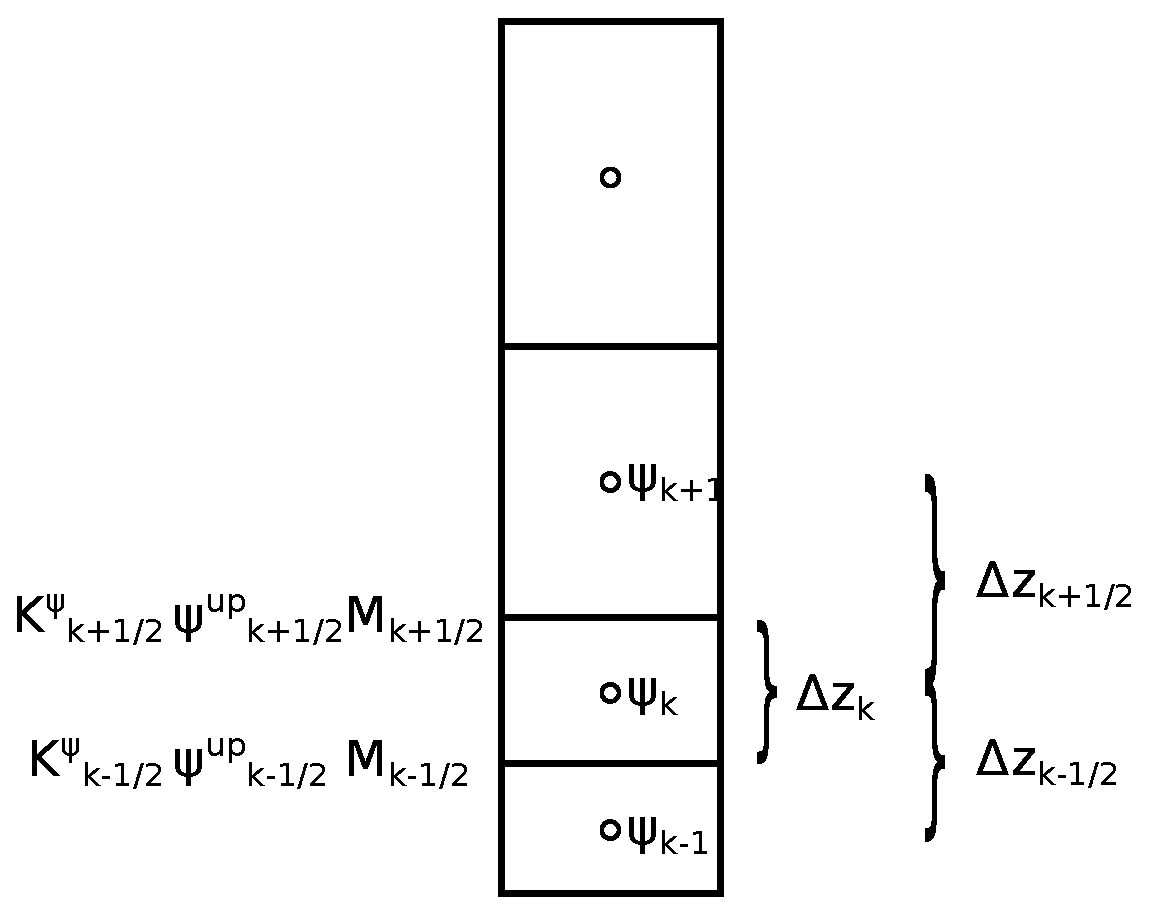
\includegraphics[width=0.5\textwidth]{staggering.eps}
\caption{Locations of prognostic variable $\psi$, the updraft mass fluxes $M_i$, the updraft properties $\psi^{up}_i$, and eddy-diffusivities $K^{\psi}$ on the 1D vertical grid. } \label{fig:staggering}
\end{figure}



\section{Cloud cover and interaction with radiation}\label{sec:clouds}

\subsection{Cumulus-topped PBL}

\subsection{Stratocumulus-topped PBL}



\section{Acknowledgements}
W.L. would like to thank Joao Teixeira and Kay Suselj for providing the code of their most recent version of the multiplume model. 


\bibliographystyle{ametsoc}
\documentclass[dvipdfmx,a4paper,10pt]{article}
\usepackage[dvips]{graphicx}
\usepackage{subfigure}
\usepackage[small,bf]{caption}
\usepackage{color}
\usepackage{natbib,amsmath}
\usepackage[margin=2.5cm]{geometry}
\usepackage{hyperref}
\hypersetup{
  colorlinks = true,
  citecolor=red,%
  filecolor=red,%
  linkcolor=red,%
  urlcolor=red
  pdfsubject = {Report},
  pdfpagemode = UseNone
}

% Title Page
\title{Implementation of an EDMF boundary-layer and shallow-cumulus parameterization into CAMR}
\author{Wolfgang Langhans}


\begin{document}
\maketitle

\section{Introduction}\label{se:intro}

For any prognostic variable $\rho\psi$ we seek to represent its tendency due to unresolved turbulent transport. Thereby, $\psi$ is one of $u$, $v$, $\theta_v$, $q_v$, and eventually $e$ (i.e., TKE).\footnote{Turbulent kinetic energy $e$ is included here since -- depending on the applied eddy-diffusivity model -- a prognostic equation for $e$ has eventually to be solved.} Here, $q_v$ is defined as the mass of water vapor per mass of moist air, as $q_v=\rho_v/(\rho_d+\rho_v)$. It is common in GCMs and mesoscale models to assume that the vertical velocity $w$ has no tendency from subgrid-scale transport. On top of that, subgrid transport is assumed to be vertical only. 

The air density $\rho=\rho_d+\rho_v$ is affected from turbulent mixing since the moisture content changes. The updated values of $\rho$, $\rho_v$, and any other variable $\rho \psi$ are obtained as 
\begin{eqnarray}
\rho^{n+1}&=&\rho^n + \Delta t \frac{\partial \rho}{\partial t}=\rho^n + \Delta t \frac{\partial \rho_v}{\partial t}=\rho^n + \Delta t \rho_d^n\left(\frac{\partial r_v}{\partial t}\right)_{turb} \\
\rho_v^{n+1}&=&\rho_v^n + \Delta t \rho_d^n\left(\frac{\partial r_v}{\partial t}\right)_{turb}\\
 (\rho\psi)^{n+1} &=& \rho^{n+1}\left[\psi^n + \Delta t \left(\frac{\partial \psi}{\partial t}\right)_{turb}\right]\\
\end{eqnarray}
whereby we used the fact that the density of dry air $\rho_d=\frac{1-q_v}{q_v}\rho_v$ remains unchanged (i.e., we are only adding/removing water vapor molecules). Here $r_v=q_v/(1-q_v)$ is the mixing ratio of water vapor.  

The tendency for any variable $\psi$ (other than $r_v$) is then obtained from the EDMF equation as
\begin{equation}\label{eqn:tendency}
 \left(\frac{\partial \psi}{\partial t}\right)_{turb} =-\frac{1}{\rho}\frac{\partial }{\partial z} \rho \left( ED^{\psi} + MF^{\psi}\right) = -\frac{1}{\rho}\frac{\partial }{\partial z} \rho\left( -K_{\psi}(z)\frac{\partial \psi(z)}{\partial z} + \sum_i M_i(z) (\psi^{up}_i(z) - \psi(z) )\right)
\end{equation}
and the tendency for $r_v$ is analogously obtained with $\rho$ replaced by $\rho_d$. Here, ED is the eddy-diffusivity part and MF the mass-flux part of the turbulent flux. Closure is provided by specifying $K_{\psi}$ and $a_i$, $w^{up}_i$, and $\psi^{up}_i$ for each updraft $i$.

The necessary/provided input to the EDMF parameterization is listed in section \ref{sec:input}. The closure is described in section \ref{sec:closure}. The numerical procedure to solve Eq. (\ref{eqn:tendency}) is outlined in section \ref{sec:solve}. One key advantage of this multiplume EDMF parameterization is that PBL mixing and shallow cumulus cloud cover are parameterized in a unified fashion. For this reason, several versions of EDMF also provide a subgrid-scale cloud cover (cumulus and eventually strato-cumulus) and cloud liquid water content which is then passed on to the radiative transfer code. The approach taken in this implementation is described in section \ref{sec:clouds}.

\section{Input}\label{sec:input}

\subsection{From CAMR Dycore}

The prognostic variables $u$, $v$, $w$, $\theta_v$, $q_v$ and $\rho$ are provided at cell centers. In this 1D framework let index $k$ represent the vertical center of cell $k$. Let indices $k-1/2$ and $k+1/2$ indicate the position of the bottom and top interface of cell $k$. Thus, the input is $u^k$, $v^k$, $w^k$, $\theta_v^k$, $q_v^k$, and $\rho_k$ with $k$ ranging from $1$ to the total number of cells $N_k$ in the 1D column. On top of that, $\rho^{k\pm 1/2}$ will be needed from the Dycore. 

Also needed for the parameterization of eddy diffusivities is the squared characteristic rate of strain $\overline{D}^2$ (based on grid-scale velocities) as defined in Eq.~(\ref{eqn:def2}) at cell centers. 

\subsection{From surface flux parameterization}\label{sec:sfcfluxes}

The parameterization of surface fluxes over ocean surface is based on \cite{bryan03} and has been used also in SAM \citep{khairou03} and CAM \citep[see][section 4.10.2]{collins04}. A formulation for fluxes over land is also available but not yet included. The formulation is adapted here to our needs as explained below. A bulk drag/transfer law is used for the surface turbulent fluxes of $u$, $v$, $\theta$, and $r_v$, given as
\begin{equation}\label{eqn:fluxes}
 (\mathbf{\tau}, E, H)=-\rho_1|\mathbf{v_h}_1| (C_d \mathbf{v_h}_1, C_e \Delta r_v, C_{\theta} \Delta \theta )
\end{equation}
with $\Delta r_v=r_{v1}-r_v^*(T_s)$, $\Delta \theta=\theta_{1}-\theta_{s}$, $\mathbf{v_h}$ the horizontal wind vector, and $C_d$, $C_e$, and $C_{\theta}$ the transfer coefficients for momentum, $r_v$, and $\theta$. $T_s$ is the surface temperature and $r_v^*(T_s)$ the saturation mixing ratio at the surface temperature. Index ``$1$'' indicates values on the first model level. 

Turbulent velocity scales $u_*$, $r_{v*}$, and $\theta_{*}$ are introduced in the formulation of these fluxes as 
\begin{eqnarray}
 u_*&=& (\overline{u'w'}^2+\overline{v'w'}^2)^{1/4} = C_d^{1/2} | \mathbf{v_h}_1 |\\
 r_{v*}&=& -\overline{r_v'w'}/u_*=C_e |\mathbf{v_h}_1| \Delta r_v / u_*\label{eqn:velqv}
\end{eqnarray}

The parameterization characterizes the surface layer stability based on the Monin-Obukhov length and then distinguishes between flux profiles for stable and unstable conditions. The parameterization proceeds by utilizing similarity theory to determine the drag coefficients $C_d$, $C_e$, and $C_{\theta}$ and the respective fluxes. That is, the parameterization provides the sensible heat flux.  Note that here we seek a flux of $\theta_v$. The required flux in kinematic units is obtained as 
\begin{equation}\label{eqn:wthetav}
 \overline{\theta_v'w'}\approx \overline{\theta'w'}(1+0.61q_{v1}) + 0.61 \theta_1  \overline{r_v'w'}.
\end{equation}
This approximation implied dropping the contribution from the triple-correlation $\overline{w'q_v'\theta'}$ \citep[same as in Eq.~(10) in][]{stull94}. However, note that the flux of virtual potential temperature is commonly even further approximated as $\overline{\theta_v'w'}=\overline{\theta'w'}+0.61 \theta_1  \overline{r_v'w'}$ \citep[e.g.,][Eq.~(10.11)]{wyngaard10}. 

Using the bulk transfer law $H_v=-\rho_1|\mathbf{v_h}_1| C_{\theta_v}\Delta \theta_{v}$ and setting this equal to the flux obtained through (\ref{eqn:wthetav}) yields 
\begin{equation}\label{eqn:dragvirtual}
C_{\theta_v}=(C_h\Delta \theta [1+0.61q_{v1}] + 0.61 C_e\theta_1\Delta r_v)/ \Delta \theta_{v}. 
\end{equation}



\section{EDMF closure}\label{sec:closure}

The task of the parameterization is to provide the eddy diffusivities $K_{\psi}$ and $a_i$, $w^{up}_i$, and $\psi^{up}_i$ for each updraft $i$. For this implemetation, we decided to start by parameterizing the eddy diffusivities using 1-dimensional closures, either a Smagorinsky or a TKE closure. Both have been adapted and modified from SAM. The updraft properties are obtained through a multiplume model that was kindly provided by Kay Suselj/JPL.


\subsection{Eddy-diffusivity models}

Same as in SAM, the eddy diffusivities are computed at cell centers and averaging provides $K_{\psi}^{k\pm 1/2}$ at cell interfaces. 

\subsubsection{Smagorinsky closure}

This LES closure relates the eddy diffusivity for momentum to the characteristic rate of strain $\overline{D}$, as
\begin{equation}\label{eqn:viscosity}
K_m=(c_s l)^2 \overline{D}\sqrt{\max\left(0,1-\frac{\mathrm{Ri}}{\mathrm{Ri}_{c}}\right)}
\end{equation}
with the Richardson number defined as 
\begin{equation}
 \mathrm{Ri}=\left\{
\begin{array}{ll}
N_m^2/\overline{D}^2&\mathrm{for~saturated~air}\\
N^2/\overline{D}^2&\mathrm{for~unsaturated~air}.
\end{array}
\right.  
\end{equation} 
and $\mathrm{Ri}_c=1.0$ a critical Richardson number and $N$ and $N_m$ the Brunt-V\"{a}is\"{a}l\"{a} frequencies in unsaturated and saturated air, respectively. Air is defined saturated if the mixing ratio of non-precipitating condensate is larger than a certain threshold. Equation (\ref{eqn:viscosity}) can be rewritten as 
\begin{equation}
K_m=(c_s l)^2 \sqrt{\max\left(0,\overline{D}^2-\frac{N^2}{\mathrm{Ri}_{c}}\right)}
\end{equation}
and equivalently using $N_m^2$ in case of saturated air (only $N^2$ is used for brevity below). The mixing length scale $l$ is stability dependent and expressed as
\begin{equation}\label{eqn:lmixsmag}
 l=\left\{ 
 \begin{array}{ll}
 \min(\Delta z, \max(0.1\Delta z, 0.76 \sqrt{(e/N^2)}))&\quad \mathrm{if}\quad N^2>0\\
 \Delta z &\quad \mathrm{if}\quad N^2\leq 0.
 \end{array}
\right.  
\end{equation}
with $e$ the TKE distribution from the previous timestep that (ideally) got advected by the Dycore. TKE is diagnosed as $e = (K_m/(c_kl))^2$. The constant $c_s$ is given through the relation $c_s^4=c_k^3/c_e$ with $c_k=0.1$ and $c_e=0.54+1.44 l/\Delta z$. The eddy diffusivity for scalar transport is obtained as $K_h=\mathrm{Pr}K_m$ with the Prandtl number set to $\mathrm{Pr}=1/\mathrm{Ri}_c=1$. 

The square of the characteristic rate of strain $\overline{D}^2$ is defined as $\overline{D}^2=2D_{ij}D_{ij}$ with element $(i,j)$ of the tensor given as
\begin{equation}
 D_{ij}=\frac{1}{2}(\frac{\partial U_i}{\partial x_j}+\frac{\partial U_j}{\partial x_i})
\end{equation}
with capital $U$ indicating the grid-scale velocity and indices $i$ and $j$ are one of the three coordinate directions. After summation one obtains 
\begin{equation}\label{eqn:def2}
 \overline{D}^2=2\{D_{11}^2+D_{22}^2+D_{33}^2\}+4\{D_{12}^2+D_{13}^2+D_{23}^2 \}
\end{equation}
which is provided from the Dycore at cell centers. 


\subsubsection{TKE closure}
The formulation of the TKE boundary layer scheme follows the description given by \cite{teixeira04} and is specifically designed here to model the evolution of the convective boundary layer (and not as a LES closure). The prognostic equation for $e$, the sgs kinetic energy per unit dry air, is
\begin{eqnarray}\label{eqn:tkebudget}
 \frac{\partial e}{\partial t}&=& \mathrm{ADV} + \mathrm{TRANS} + \mathrm{SHEAR} + \mathrm{BUOY} - \mathrm{DISS}\\
 \mathrm{TRANS} &=& \frac{1}{\rho_d}\frac{\partial}{\partial z} (\rho_d K_m  \frac{\partial e}{\partial z})\\
 \mathrm{SHEAR} &=& K_m \overline{D}^2 \\
 \mathrm{BUOY} &=& \frac{g}{\theta_v}\overline{w'\theta_v'}\\
 \mathrm{DISS}&=& 0.16\cdot 2.5\sqrt{e}/l.
\end{eqnarray}
The virtual potential temperature flux is the sum of the ED and MF parts and computed at the end of the previous time step. The advective term is eventually computed by the Dycore which has TKE per mass of moist air as prognostic variable such that conversion is required (i.e., analogous to the water vapor mixing ratio). The eddy diffusivity for momentum is obtained as $K_m=0.5 l \sqrt{e}$ and $K_h=\mathrm{Pr} K_m$ with $\mathrm{Pr}=1$. The mixing length is obtained as
\begin{eqnarray}
 l &=& \tau \sqrt{e} + (\kappa z - \tau \sqrt{e}) e^{-z/\alpha}
\end{eqnarray}
with $\alpha=100\mathrm{~m}$ and $\tau$ taken to be either 600 sec or $\tau=h/w^*$ with $w^*=(hg/\theta_{v0} \overline{w'\theta_v'})^{1/3}$. The boundary layer height $h$ is defined as the level where the buoyancy flux is minimized. The TRANS diffusion term is solved in the same way as for any other scalar. Note that to obtain a standard LES TKE closure the mixing length can be defined same as in (\ref{eqn:lmixsmag}) and the coefficients in DISS can be adopted. 

The numerical implementation to advance $e$ from step $n$ to step $n+1$ is as follows. SHEAR, BUOY, and DISS are treated explicitly with an Euler step. Thereby, $K_m$ at step $n$ is diagnosed from $e$ at step $n$. In case the boundary layer height $h$ (defined as the level where the buoyancy flux is minimized) and $w^*$ are needed to evaluate mixing length $l$, the required buoyancy flux is obtained from the implicit computation for the previous time step. The three tendencies will be limited in magnitude to ensure their sum is not smaller than $-\frac{e}{\Delta t}$. Then, TRANS is computed as described below (general formulation allowing for an implicit solver) again based on the $e$ distribution at step $n$. That means that TRANS may still cause some negative $e$ at step $n+1$ since the solver for TRANS is not necessarily positive definite. Negative $e$ will be clipped at the beginning of the next step.   

\subsection{Multiplume model}

\subsubsection{Description}

The multiplume model provides updarft properties for a user-set number of plumes and thus the MF-part in Eq.~(\ref{eqn:tendency}). It closely follows the proposed multiplume model of \cite{cheinet03a}. Each plume represents one class of updrafts with the same thermodyniamic and kinematic properties. Note that in Eq.~(\ref{eqn:tendency}) it has been assumed that $\psi_d$ of the undisturbed subsiding air in the environment equals the grid-box mean $\psi$. This is equivalent to assuming that the updraft/downdraft area is small. This assumption is not made in, e.g., \cite{cheinet03a}. Following \cite{suselj12}, \cite{suselj13}, and \cite{suselj14} the MF part is assumed to be zero in case of $\psi$ equal to $u$, $v$, or $e$. This is generally justified by the smaller eddy viscosities for momentum than for heat and the general lack in knowledge about sources/sinks of momentum within a rising plume \citep[see, e.g., discussion in][]{han15}. Index $i$ identifies an individual updraft class among a total of $N^{up}$ (to be specified, e.g., $N^{up}=10$) updrafts. $M_i$ is defined as $s_i w^{up}_i$ with $s_i$ and $w^{up}_i$ the fractional weight and vertical velocity, respectively, of updraft class $i$. 


Initial conditions are obtained as in \cite{cheinet03a} and \cite{lenschow80}. Through similarity theory the initial conditions are linked to surface fluxes, boundary layer depth, and an assumed PDF of the vertical velocity. The latter is assumed to be a Gaussian with standard deviation $\sigma_w$, given as

\begin{equation}
 f_w(w) = \frac{1}{\sigma_w 2 \pi } e^{-\frac{w^2}{2\sigma_w^2}}.
\end{equation}


A fixed number of plumes spans a discrete PDF for a selected range between $w_{\mathrm{min}}$ and $w_{\mathrm{max}}$. Plume $i$ covers all vertical velocities between

\begin{eqnarray}
 w_i^{\mathrm{min}}&=&w_{\mathrm{min}}+(i-1)(w_{\mathrm{max}}-w_{\mathrm{min}})/N^{up} \qquad\mathrm{and}\\
 w_i^{\mathrm{max}}&=&w_{\mathrm{min}}+i(w_{\mathrm{max}}-w_{\mathrm{min}})/N^{up},
\end{eqnarray}
has a fractional weight  
\begin{equation}
 s_i =1/2(\mathrm{erf}(\frac{w_i^{\mathrm{max}}}{\sqrt{2}\sigma_w}) - \mathrm{erf}(\frac{w_i^{\mathrm{min}}}{\sqrt{2}\sigma_w})),
\end{equation}
and an average initial updraft velocity of 
\begin{equation}
 w_i =   \frac{\sigma_w}{s_i \sqrt{2 \pi }} (e^{-\frac{{w_i^{\mathrm{min}}}^2}{2 \sigma_w^2}}- e^{-\frac{{w_i^{\mathrm{max}}}^2}{2 \sigma_w^2}}).
\end{equation}
This initial average velocity has been modified here from the original $1/2(w_i^{\mathrm{min}}+w_i^{\mathrm{max}})$ used by Kay/JPL in order to make sure that the total upward mass flux $\rho \int\limits_0^{\infty} dw~f_w w = \rho \int\limits_0^{\infty} ds~ w=\rho \sum_{i=1,N_p} s_i w_i $ is independent of $N_p$. To illustrate the difference, if $w_{\mathrm{min}}=0$ and $w_{\mathrm{max}}\gg\sqrt{2}\sigma_w$ then the total area covered by updrafts is 0.5. Then, if only one plume was used, the average initial velocity would be $w_1=\sqrt{\frac{2}{\pi}} \sigma_w$ and not $0.5 w_i^{\mathrm{max}}$ as in the unmodified code. This update should allow for better convergence characteristics with an increasing number of plumes. 


The actual physical area fraction $f_i$ of a class spanned between $w_i^{\mathrm{min}}$ and $w_i^{\mathrm{max}}$ results from 
$\int\limits_{w_i^{\mathrm{min}}}^{w_i^{\mathrm{max}}} dw~ f(w) =\frac{1}{A_{tot}}\int\limits dA~N^*_i a_i$ with $N^*_i$ the number density (m$^{-2}$) and $a_i$ the areal extent of updrafts with velocities in the range $w_i^{\mathrm{min}}<w<w_i^{\mathrm{max}}$. The distributions $N^*_i(x,y)$ and $a_i(x,y)$ are defined to be zero whenever $w(x,y)$ falls outside of the specified range of the class. Of course, we can try and assume that all updrafts in one class have the same size such that 

\begin{equation}
 f_i = \frac{\int\limits_{w_i^{\mathrm{min}}}^{w_i^{\mathrm{max}}} dw~ f(w) }{ \int\limits_{A_{tot}} dA~N^*_i}= \frac{s_i }{ N_i}.
\end{equation}

Specifying $s_i$ thus leaves us to specify either the total number of updrafts represented by class $i$ or their fractional area $f_i$, but obviously not both.

Initial thermodynamic properties are obtained through similarity relations, as 
\begin{eqnarray}
 q_{vi}&=&q_{v}+0.32 w_i  \sigma_{q_t}/\sigma_w\\
 \theta_{vi}&=&\theta_{v}+0.58 w_i  \sigma_{\theta_v}/\sigma_w\\
  \theta_{li}&=&\theta_{vi}/(1+\epsilon q_{vi})=\theta_i \quad\mathrm{since}~q_{li}=0\\
  w^*&=&(hg/\theta_v \overline{w'\theta_v'})^{1/3}\\
  q_v^*&=&\overline{w'q_v'}/w^*\\
  \theta_v^*&=&\overline{w'\theta_v'}/w^*\\
 \sigma_w&=&1.34 w^*(z_s/h)^{1/3} (1-0.8z_s/h)\\
   \sigma_{q_t}&=&1.34 q_v^* (z_s/h)^{-1/3}\\
  \sigma_{\theta_v}&=&1.34\theta_v^* (z_s/h)^{-1/3}
\end{eqnarray}
with coefficients chosen in agreement with \cite{lenschow80} and the boundary layer height $h$ defined as the level where the buoyancy flux gets minimized. $z_s$ is set to be 50 meter and supposed to be in the surface layer. 

Steady-state plumes are used to describe the vertical profile of the properties in entraining and ascending parcels. A conserved quantity $\psi$ follows the vertical profile given by
\begin{eqnarray}\label{eqn:conserved}
 \frac{d\psi_i^{up} }{d z } &=& - \epsilon(\psi_i^{up} - \psi)
\end{eqnarray}
with entrainment rate $\epsilon$ and the environmental value $\psi$. The parcel rises until its vertical velocity reaches zero. The latter is given by
\begin{eqnarray}\label{eqn:w}
 \frac{d (w_i^{up})^2 }{d z } &=& 2aB^{up}_i- (2b+c\epsilon)(w_i^{up})^2
\end{eqnarray}
with buoyancy $B_i^{up}=g(\theta_v^{up}/\theta_v-1)$, the environmental profile $\theta_v$, and constants $a$, $b$, and $c$. The three acceleration terms are buoyancy, form drag, and mixing drag. 


The conserved variables used in the plume equations are liquid water potential temperature $\theta_l$ and total water mass fraction $q_t=q_v+q_l$. Equation (\ref{eqn:conserved}) is solved for these two variables until the vertical velocity in a plume turns zero. At each height a saturation adjustment scheme is used to infer the liquid water content $q_l$, $q_v$, and $\theta_v$. 


\subsubsection{Discretization}
Solving the vertical velocity and scalar equation in the vertical is accomplished as in \cite{suselj14} (see their appendix). Thereby we assume that $\epsilon$, the environment value $\psi$, and buoyancy $B$ can be considered constant in each layer (instead of, e.g., $\epsilon(\psi^{up}-\psi)$ being constant) to obtain an analytical expression for $\psi$ at the next level. This method has the numerical advantage that $\psi^{up}$ at the next higher level will be bound in between the value of $\psi^{up}$ at the lower level and the environmental value of $\psi$ in that layer. This provides the mass flux properties ($M_i^{k\pm 1/2}$ and $\psi^{up~k\pm 1/2}_i$) on cell interfaces. The discretized equations are 
\begin{eqnarray}
 \psi_i^{up~k+1/2}&=&\psi^{~k}(1-e^{-\epsilon^{k}\Delta z^k})+\psi_i^{up~k-1/2}e^{-\epsilon^{k}\Delta z^k}\\
 (w_i^{up~k+1/2})^2&=&(\alpha w_i^{up~k-1/2})^2 + (1-\alpha^2) \frac{aB_i^{up~k}}{b+c\epsilon^k},
\end{eqnarray}
where $\alpha=e^{-(b+c\epsilon^k)\Delta z^k}$ and $B_i^{up~k}=g(0.5(\theta_{vi}^{up~k+1/2}+\theta_{vi}^{up~k-1/2})/\theta_v^{k}-1)$. The entrainment rate (m$^{-1}$) in layer $\Delta z^k$ is computed as
\begin{equation}
 \epsilon(\Delta z^k) = \frac{1}{\Delta z^k} \epsilon_d \mathcal{P}(\frac{\Delta z^k}{L_0})
\end{equation}
with $\epsilon_d=0.1$, $L_0=100$~m, $a=2/3$, $b=0.002$~m$^{-1}$, $c=1.5$, and $\mathcal{P}$ a random number drawn from the Poisson distribution. The entrainment rate is thus so far formulated identically for the different updraft classes. 

\section{Solving for the tendency}\label{sec:solve}

Equation (\ref{eqn:tendency}) needs to be solved to obtain tentendy $T^{\psi}$. The spatial discretization of the equations is done using a centered scheme for the diffusion term and the mass-flux term. Same as in Teixeira and Siebesma (2000), \cite{siebesma07}, and \cite{soares04}, disretization in time is achieved using a fully implicit scheme for both the diffusion and the mass flux term. $K$, $M_i$, and $\psi^{up}_i$ are treated explicitly in time.\footnote{If the prognostic TKE closure is used then SAM would use an intermediate $K$ obtained from an intermediate $e$ that got advanced through a truncated budget (\ref{eqn:tkebudget}) without the TRANS term. TRANS (i.e. mixing) is then computed based on the intermediate $e$ and $K$. We find, however, that this approach leads to strange instabilities in a CPBL test. Thus, we use a truly explicit approach for $e$ and $K$.} See the discussion in \cite{siebesma07} (section 4c and appendix B) for further reference. For brevity we drop index $_\psi$ here for eddy diffusivities $K$. The vertical grid structure and the indexing is illustrated in Fig.~\ref{fig:staggering}. The discretized form of Eq. (\ref{eqn:tendency}) is
\begin{align*}
  &\frac{\psi^{n+1,k}- \psi^{n,k} }{\Delta t} =\\
  &-\frac{1}{\rho^{n,k}\Delta z^{k}}\left\{ -\frac{K^{n,k+1/2}\rho^{n,k+1/2} }{\Delta z^{k+1/2}} [\beta_1^+(\psi^{n+1,k+1}-\psi^{n+1,k}) + \beta_1^-(\psi^{n,k+1}-\psi^{n,k})] \right. \\
    & \left.+\frac{K^{n,k-1/2}\rho^{n,k-1/2} }{\Delta z^{k-1/2}} [\beta_1^+(\psi^{n+1,k}-\psi^{n+1,k-1}) + \beta_1^-(\psi^{n,k}-\psi^{n,k-1})] \right.\\
    & \left. +\rho^{n,k+1/2}\left[\sum_i M_i^{n,k+1/2}\psi_i^{up~n,k+1/2} - \frac{1}{2}(\beta_2^+\psi^{n+1,k}+\beta_2^-\psi^{n,k}+\beta_2^+\psi^{n+1,k+1}+\beta_2^-\psi^{n,k+1} )\sum_i M_i^{n,k+1/2} \right]\right.\\
    &\left.-\rho^{n,k-1/2}\left[\sum_i M_i^{n,k-1/2}\psi_i^{up~n,k-1/2} - \frac{1}{2}(\beta_2^+\psi^{n+1,k}+\beta_2^-\psi^{n,k}+\beta_2^+\psi^{n+1,k-1}+\beta_2^-\psi^{n,k-1} )\sum_i M_i^{n,k-1/2} \right] \right\}\\
\end{align*}
with $\beta_1^+=1-\beta_1^-$ and $\beta_2^+=1-\beta_2^-$ the implicit weights. A fully implicit solver, i.e., $\beta_1^{+}=\beta_2^{+}=1$, is used here to prevent instabilities. A tridiagonal matrix solver is used to solve $\mathbf{A}\cdot\Psi^{n+1}=\mathbf{d}$ for $\Psi^{n+1}$. 

\noindent For $2\leq k \leq N_k-1$ the coefficients are given as 

\begin{align*}
  a_k &=  \frac{\rho^{n,k-1/2}}{\rho^{n,k}\Delta z^k} \left[\beta_1^+ \frac{K^{n,k-1/2}}{\Delta z ^{k-1/2}}-\beta_2^+\frac{1}{2} \sum_iM_i^{n,k-1/2}\right]\\
    b_k &= -\frac{1}{\Delta t} + \frac{\rho^{n,k+1/2}}{\rho^{n,k}\Delta z^k} \left[-\beta_1^+\frac{K^{n,k+1/2}}{\Delta z ^{k+1/2}}+\beta_2^+\frac{1}{2}\sum_iM_i^{n,k+1/2} \right]-\frac{\rho^{n,k-1/2}}{\rho^{n,k}\Delta z^k} \left[\beta_1^+\frac{K^{n,k-1/2}}{\Delta z ^{k-1/2}}+\beta_2^+\frac{1}{2}\sum_iM_i^{n,k-1/2} \right] \\
      c_k &= \frac{\rho^{n,k+1/2}}{\rho^{n,k}\Delta z^k}\left[\beta_1^+ \frac{K^{n,k+1/2}}{\Delta z ^{k+1/2}}+\beta_2^+\frac{1}{2}\sum_iM_i^{n,k+1/2} \right] \\
      d_k &=-\frac{\psi^{n,k}}{\Delta t} - \frac{1}{\rho^{n,k}\Delta z^k} \left\{ \frac{K^{n,k+1/2}\rho^{n,k+1/2}}{\Delta z^{k+1/2}}\beta_1^{-}\left[\psi^{n,k+1} - \psi^{n,k}\right]-\frac{K^{n,k-1/2}\rho^{n,k-1/2}}{\Delta z^{k-1/2}}\beta_1^{-}\left[\psi^{n,k} - \psi^{n,k-1}\right]\right.   \\   
          & \left.+\rho^{n,k-1/2}\left[\sum_iM_i^{n,k-1/2}\psi_i^{up~n,k-1/2} - \frac{1}{2}\beta_2^{-}(\psi^{n,k}+\psi^{n,k-1})\sum_iM_i^{n,k-1/2} \right]\right.\\
          & \left. -\rho^{n,k+1/2}\left[\sum_iM_i^{n,k+1/2}\psi_i^{up~n,k+1/2} - \frac{1}{2}\beta_2^{-}(\psi^{n,k}+\psi^{n,k+1})\sum_iM_i^{n,k+1/2} \right] \right\}.
\end{align*}

\noindent The boundary conditions at the surface are specified for $k=1$, as

\begin{align*}
  a_k &= 0 \\
    b_k &= -\frac{1}{\Delta t} +\frac{\rho^{n,k+1/2}}{\rho^{n,k}\Delta z^k} \left[- \beta_1^+\frac{K^{n,k+1/2}}{\Delta z^{k+1/2}}+ \beta_2^+\frac{1}{2}\sum_iM_i^{n,k+1/2} \right]-\beta_1^+|\mathbf{v_{h1}}|C^n_{\psi}/\Delta z^k  \\
      c_k &= \mathrm{same~as~for~}2\leq k \leq N_k-1 \\
      d_k &=  -\frac{\psi^{n,k}}{\Delta t} - \frac{1}{\rho^{n,k}\Delta z^k} \left\{ \frac{K^{n,k+1/2}\rho^{n,k+1/2}}{\Delta z^{k+1/2}}\beta_1^{-}\left[\psi^{n,k+1} - \psi^{n,k}\right]\right.   \\   
          & \left. -\rho^{n,k+1/2}\left[\sum_iM_i^{n,k+1/2}\psi_i^{up~n,k+1/2} - \frac{1}{2}\beta_2^{-}(\psi^{n,k}+\psi^{n,k+1})\sum_iM_i^{n,k+1/2} \right] \right\} +|\mathbf{v_{h1}}|\frac{C^n_{\psi}}{\Delta z^k}\left[\beta^-\psi^{n,k} - \psi_s\right]    
\end{align*}
This formulation with Dirichlet boundary conditions makes use of the drag coefficients computed in the surface scheme and through (\ref{eqn:dragvirtual}). The user can, however, also decide to use a Neuman boundary condition ({\tt doneuman=.true.}) using the fluxes from the surface scheme and from (\ref{eqn:wthetav}). In this case, the last rhs term in $b_k$ is dropped and the last term in $d_k$ becomes $- \overline{\psi'w'}^n/\Delta z^k$ makeing the surface fluxes fully explicit. This explicit Neuman boundary condition is also used if surface fluxes are prescribed ({\tt sfc\_tau\_fxd} or {\tt sfc\_flx\_fxd} respectively). Same as in SAM, the surface flux of $e$ is assumed to be zero and the explicit Neuman condition is always used. 

The boundary condition at the top for $k=N_k$ is given as
\begin{align*}
  a_k &= \mathrm{same~as~for~}2\leq k \leq N_k-1  \\
    b_k &= -\frac{1}{\Delta t} - \frac{\rho^{n,k-1/2}}{\rho^{n,k}\Delta z^k} \left[\beta_1^+\frac{K^{n,k-1/2}}{\Delta z ^{k-1/2}}+\beta_2^+\frac{1}{2}\sum_iM_i^{n,k-1/2} \right] \\
      c_k &= 0 \\
      d_k &= -\frac{\psi^{n,k}}{\Delta t} + \frac{1}{\rho^{n,k}\Delta z^k} \left\{ \frac{K^{n,k-1/2}\rho^{n,k-1/2}}{\Delta z^{k-1/2}}\beta_1^{-}\left[\psi^{n,k} - \psi^{n,k-1}\right]\right.   \\   
          & \left.-\rho^{n,k-1/2}\left[\sum_iM_i^{n,k-1/2}\psi_i^{up~n,k-1/2} - \frac{1}{2}\beta_2^{-}(\psi^{n,k}+\psi^{n,k-1})\sum_iM_i^{n,k-1/2} \right]\right\}.    
\end{align*}
Again, $\rho$ needs to be replaced by $\rho_d$ in case of $\psi=r_v$ or $\psi=e$. 


 

\begin{figure}[bthp]
\centering
 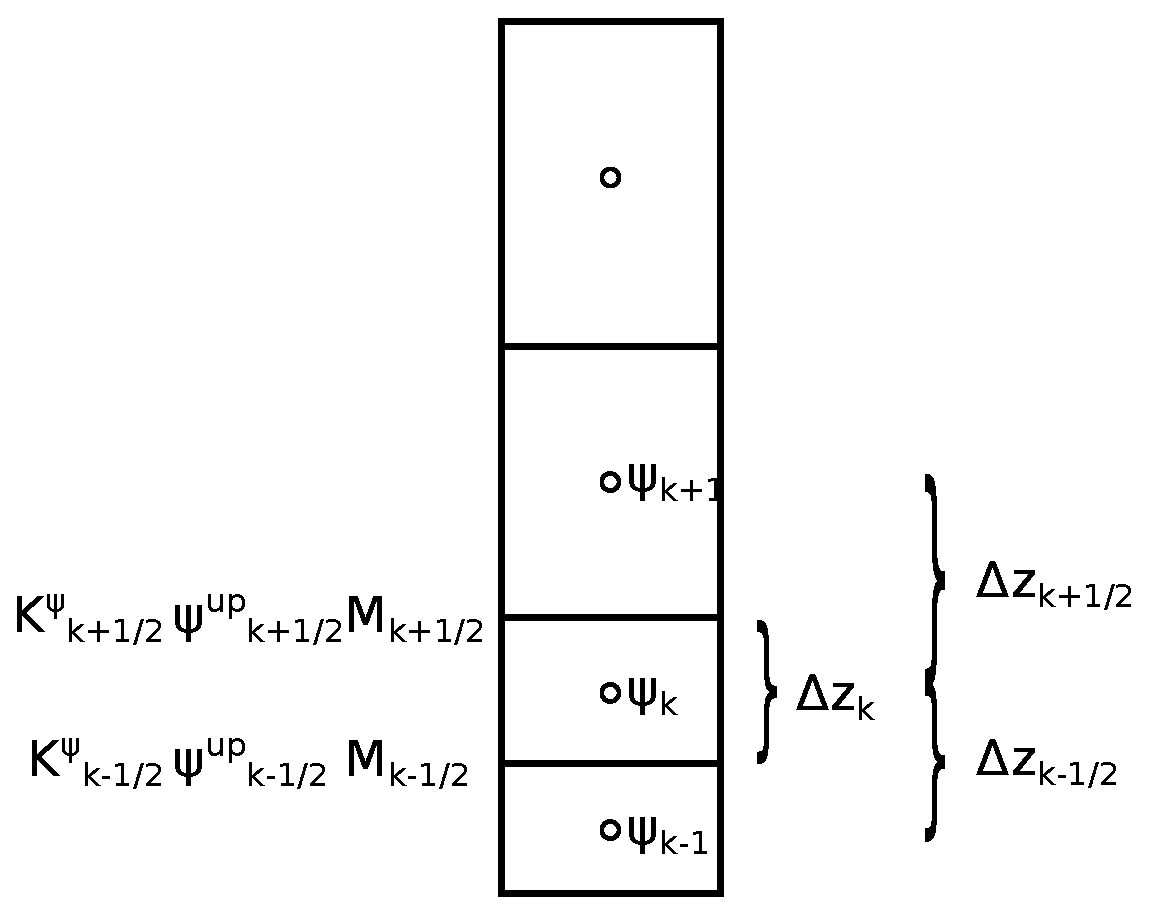
\includegraphics[width=0.5\textwidth]{staggering.eps}
\caption{Locations of prognostic variable $\psi$, the updraft mass fluxes $M_i$, the updraft properties $\psi^{up}_i$, and eddy-diffusivities $K^{\psi}$ on the 1D vertical grid. } \label{fig:staggering}
\end{figure}



\section{Cloud cover and interaction with radiation}\label{sec:clouds}

\subsection{Cumulus-topped PBL}

\subsection{Stratocumulus-topped PBL}



\section{Acknowledgements}
W.L. would like to thank Joao Teixeira and Kay Suselj for providing the code of their most recent version of the multiplume model. 


\bibliographystyle{ametsoc}
\documentclass[dvipdfmx,a4paper,10pt]{article}
\usepackage[dvips]{graphicx}
\usepackage{subfigure}
\usepackage[small,bf]{caption}
\usepackage{color}
\usepackage{natbib,amsmath}
\usepackage[margin=2.5cm]{geometry}
\usepackage{hyperref}
\hypersetup{
  colorlinks = true,
  citecolor=red,%
  filecolor=red,%
  linkcolor=red,%
  urlcolor=red
  pdfsubject = {Report},
  pdfpagemode = UseNone
}

% Title Page
\title{Implementation of an EDMF boundary-layer and shallow-cumulus parameterization into CAMR}
\author{Wolfgang Langhans}


\begin{document}
\maketitle

\section{Introduction}\label{se:intro}

For any prognostic variable $\rho\psi$ we seek to represent its tendency due to unresolved turbulent transport. Thereby, $\psi$ is one of $u$, $v$, $\theta_v$, $q_v$, and eventually $e$ (i.e., TKE).\footnote{Turbulent kinetic energy $e$ is included here since -- depending on the applied eddy-diffusivity model -- a prognostic equation for $e$ has eventually to be solved.} Here, $q_v$ is defined as the mass of water vapor per mass of moist air, as $q_v=\rho_v/(\rho_d+\rho_v)$. It is common in GCMs and mesoscale models to assume that the vertical velocity $w$ has no tendency from subgrid-scale transport. On top of that, subgrid transport is assumed to be vertical only. 

The air density $\rho=\rho_d+\rho_v$ is affected from turbulent mixing since the moisture content changes. The updated values of $\rho$, $\rho_v$, and any other variable $\rho \psi$ are obtained as 
\begin{eqnarray}
\rho^{n+1}&=&\rho^n + \Delta t \frac{\partial \rho}{\partial t}=\rho^n + \Delta t \frac{\partial \rho_v}{\partial t}=\rho^n + \Delta t \rho_d^n\left(\frac{\partial r_v}{\partial t}\right)_{turb} \\
\rho_v^{n+1}&=&\rho_v^n + \Delta t \rho_d^n\left(\frac{\partial r_v}{\partial t}\right)_{turb}\\
 (\rho\psi)^{n+1} &=& \rho^{n+1}\left[\psi^n + \Delta t \left(\frac{\partial \psi}{\partial t}\right)_{turb}\right]\\
\end{eqnarray}
whereby we used the fact that the density of dry air $\rho_d=\frac{1-q_v}{q_v}\rho_v$ remains unchanged (i.e., we are only adding/removing water vapor molecules). Here $r_v=q_v/(1-q_v)$ is the mixing ratio of water vapor.  

The tendency for any variable $\psi$ (other than $r_v$) is then obtained from the EDMF equation as
\begin{equation}\label{eqn:tendency}
 \left(\frac{\partial \psi}{\partial t}\right)_{turb} =-\frac{1}{\rho}\frac{\partial }{\partial z} \rho \left( ED^{\psi} + MF^{\psi}\right) = -\frac{1}{\rho}\frac{\partial }{\partial z} \rho\left( -K_{\psi}(z)\frac{\partial \psi(z)}{\partial z} + \sum_i M_i(z) (\psi^{up}_i(z) - \psi(z) )\right)
\end{equation}
and the tendency for $r_v$ is analogously obtained with $\rho$ replaced by $\rho_d$. Here, ED is the eddy-diffusivity part and MF the mass-flux part of the turbulent flux. Closure is provided by specifying $K_{\psi}$ and $a_i$, $w^{up}_i$, and $\psi^{up}_i$ for each updraft $i$.

The necessary/provided input to the EDMF parameterization is listed in section \ref{sec:input}. The closure is described in section \ref{sec:closure}. The numerical procedure to solve Eq. (\ref{eqn:tendency}) is outlined in section \ref{sec:solve}. One key advantage of this multiplume EDMF parameterization is that PBL mixing and shallow cumulus cloud cover are parameterized in a unified fashion. For this reason, several versions of EDMF also provide a subgrid-scale cloud cover (cumulus and eventually strato-cumulus) and cloud liquid water content which is then passed on to the radiative transfer code. The approach taken in this implementation is described in section \ref{sec:clouds}.

\section{Input}\label{sec:input}

\subsection{From CAMR Dycore}

The prognostic variables $u$, $v$, $w$, $\theta_v$, $q_v$ and $\rho$ are provided at cell centers. In this 1D framework let index $k$ represent the vertical center of cell $k$. Let indices $k-1/2$ and $k+1/2$ indicate the position of the bottom and top interface of cell $k$. Thus, the input is $u^k$, $v^k$, $w^k$, $\theta_v^k$, $q_v^k$, and $\rho_k$ with $k$ ranging from $1$ to the total number of cells $N_k$ in the 1D column. On top of that, $\rho^{k\pm 1/2}$ will be needed from the Dycore. 

Also needed for the parameterization of eddy diffusivities is the squared characteristic rate of strain $\overline{D}^2$ (based on grid-scale velocities) as defined in Eq.~(\ref{eqn:def2}) at cell centers. 

\subsection{From surface flux parameterization}\label{sec:sfcfluxes}

The parameterization of surface fluxes over ocean surface is based on \cite{bryan03} and has been used also in SAM \citep{khairou03} and CAM \citep[see][section 4.10.2]{collins04}. A formulation for fluxes over land is also available but not yet included. The formulation is adapted here to our needs as explained below. A bulk drag/transfer law is used for the surface turbulent fluxes of $u$, $v$, $\theta$, and $r_v$, given as
\begin{equation}\label{eqn:fluxes}
 (\mathbf{\tau}, E, H)=-\rho_1|\mathbf{v_h}_1| (C_d \mathbf{v_h}_1, C_e \Delta r_v, C_{\theta} \Delta \theta )
\end{equation}
with $\Delta r_v=r_{v1}-r_v^*(T_s)$, $\Delta \theta=\theta_{1}-\theta_{s}$, $\mathbf{v_h}$ the horizontal wind vector, and $C_d$, $C_e$, and $C_{\theta}$ the transfer coefficients for momentum, $r_v$, and $\theta$. $T_s$ is the surface temperature and $r_v^*(T_s)$ the saturation mixing ratio at the surface temperature. Index ``$1$'' indicates values on the first model level. 

Turbulent velocity scales $u_*$, $r_{v*}$, and $\theta_{*}$ are introduced in the formulation of these fluxes as 
\begin{eqnarray}
 u_*&=& (\overline{u'w'}^2+\overline{v'w'}^2)^{1/4} = C_d^{1/2} | \mathbf{v_h}_1 |\\
 r_{v*}&=& -\overline{r_v'w'}/u_*=C_e |\mathbf{v_h}_1| \Delta r_v / u_*\label{eqn:velqv}
\end{eqnarray}

The parameterization characterizes the surface layer stability based on the Monin-Obukhov length and then distinguishes between flux profiles for stable and unstable conditions. The parameterization proceeds by utilizing similarity theory to determine the drag coefficients $C_d$, $C_e$, and $C_{\theta}$ and the respective fluxes. That is, the parameterization provides the sensible heat flux.  Note that here we seek a flux of $\theta_v$. The required flux in kinematic units is obtained as 
\begin{equation}\label{eqn:wthetav}
 \overline{\theta_v'w'}\approx \overline{\theta'w'}(1+0.61q_{v1}) + 0.61 \theta_1  \overline{r_v'w'}.
\end{equation}
This approximation implied dropping the contribution from the triple-correlation $\overline{w'q_v'\theta'}$ \citep[same as in Eq.~(10) in][]{stull94}. However, note that the flux of virtual potential temperature is commonly even further approximated as $\overline{\theta_v'w'}=\overline{\theta'w'}+0.61 \theta_1  \overline{r_v'w'}$ \citep[e.g.,][Eq.~(10.11)]{wyngaard10}. 

Using the bulk transfer law $H_v=-\rho_1|\mathbf{v_h}_1| C_{\theta_v}\Delta \theta_{v}$ and setting this equal to the flux obtained through (\ref{eqn:wthetav}) yields 
\begin{equation}\label{eqn:dragvirtual}
C_{\theta_v}=(C_h\Delta \theta [1+0.61q_{v1}] + 0.61 C_e\theta_1\Delta r_v)/ \Delta \theta_{v}. 
\end{equation}



\section{EDMF closure}\label{sec:closure}

The task of the parameterization is to provide the eddy diffusivities $K_{\psi}$ and $a_i$, $w^{up}_i$, and $\psi^{up}_i$ for each updraft $i$. For this implemetation, we decided to start by parameterizing the eddy diffusivities using 1-dimensional closures, either a Smagorinsky or a TKE closure. Both have been adapted and modified from SAM. The updraft properties are obtained through a multiplume model that was kindly provided by Kay Suselj/JPL.


\subsection{Eddy-diffusivity models}

Same as in SAM, the eddy diffusivities are computed at cell centers and averaging provides $K_{\psi}^{k\pm 1/2}$ at cell interfaces. 

\subsubsection{Smagorinsky closure}

This LES closure relates the eddy diffusivity for momentum to the characteristic rate of strain $\overline{D}$, as
\begin{equation}\label{eqn:viscosity}
K_m=(c_s l)^2 \overline{D}\sqrt{\max\left(0,1-\frac{\mathrm{Ri}}{\mathrm{Ri}_{c}}\right)}
\end{equation}
with the Richardson number defined as 
\begin{equation}
 \mathrm{Ri}=\left\{
\begin{array}{ll}
N_m^2/\overline{D}^2&\mathrm{for~saturated~air}\\
N^2/\overline{D}^2&\mathrm{for~unsaturated~air}.
\end{array}
\right.  
\end{equation} 
and $\mathrm{Ri}_c=1.0$ a critical Richardson number and $N$ and $N_m$ the Brunt-V\"{a}is\"{a}l\"{a} frequencies in unsaturated and saturated air, respectively. Air is defined saturated if the mixing ratio of non-precipitating condensate is larger than a certain threshold. Equation (\ref{eqn:viscosity}) can be rewritten as 
\begin{equation}
K_m=(c_s l)^2 \sqrt{\max\left(0,\overline{D}^2-\frac{N^2}{\mathrm{Ri}_{c}}\right)}
\end{equation}
and equivalently using $N_m^2$ in case of saturated air (only $N^2$ is used for brevity below). The mixing length scale $l$ is stability dependent and expressed as
\begin{equation}\label{eqn:lmixsmag}
 l=\left\{ 
 \begin{array}{ll}
 \min(\Delta z, \max(0.1\Delta z, 0.76 \sqrt{(e/N^2)}))&\quad \mathrm{if}\quad N^2>0\\
 \Delta z &\quad \mathrm{if}\quad N^2\leq 0.
 \end{array}
\right.  
\end{equation}
with $e$ the TKE distribution from the previous timestep that (ideally) got advected by the Dycore. TKE is diagnosed as $e = (K_m/(c_kl))^2$. The constant $c_s$ is given through the relation $c_s^4=c_k^3/c_e$ with $c_k=0.1$ and $c_e=0.54+1.44 l/\Delta z$. The eddy diffusivity for scalar transport is obtained as $K_h=\mathrm{Pr}K_m$ with the Prandtl number set to $\mathrm{Pr}=1/\mathrm{Ri}_c=1$. 

The square of the characteristic rate of strain $\overline{D}^2$ is defined as $\overline{D}^2=2D_{ij}D_{ij}$ with element $(i,j)$ of the tensor given as
\begin{equation}
 D_{ij}=\frac{1}{2}(\frac{\partial U_i}{\partial x_j}+\frac{\partial U_j}{\partial x_i})
\end{equation}
with capital $U$ indicating the grid-scale velocity and indices $i$ and $j$ are one of the three coordinate directions. After summation one obtains 
\begin{equation}\label{eqn:def2}
 \overline{D}^2=2\{D_{11}^2+D_{22}^2+D_{33}^2\}+4\{D_{12}^2+D_{13}^2+D_{23}^2 \}
\end{equation}
which is provided from the Dycore at cell centers. 


\subsubsection{TKE closure}
The formulation of the TKE boundary layer scheme follows the description given by \cite{teixeira04} and is specifically designed here to model the evolution of the convective boundary layer (and not as a LES closure). The prognostic equation for $e$, the sgs kinetic energy per unit dry air, is
\begin{eqnarray}\label{eqn:tkebudget}
 \frac{\partial e}{\partial t}&=& \mathrm{ADV} + \mathrm{TRANS} + \mathrm{SHEAR} + \mathrm{BUOY} - \mathrm{DISS}\\
 \mathrm{TRANS} &=& \frac{1}{\rho_d}\frac{\partial}{\partial z} (\rho_d K_m  \frac{\partial e}{\partial z})\\
 \mathrm{SHEAR} &=& K_m \overline{D}^2 \\
 \mathrm{BUOY} &=& \frac{g}{\theta_v}\overline{w'\theta_v'}\\
 \mathrm{DISS}&=& 0.16\cdot 2.5\sqrt{e}/l.
\end{eqnarray}
The virtual potential temperature flux is the sum of the ED and MF parts and computed at the end of the previous time step. The advective term is eventually computed by the Dycore which has TKE per mass of moist air as prognostic variable such that conversion is required (i.e., analogous to the water vapor mixing ratio). The eddy diffusivity for momentum is obtained as $K_m=0.5 l \sqrt{e}$ and $K_h=\mathrm{Pr} K_m$ with $\mathrm{Pr}=1$. The mixing length is obtained as
\begin{eqnarray}
 l &=& \tau \sqrt{e} + (\kappa z - \tau \sqrt{e}) e^{-z/\alpha}
\end{eqnarray}
with $\alpha=100\mathrm{~m}$ and $\tau$ taken to be either 600 sec or $\tau=h/w^*$ with $w^*=(hg/\theta_{v0} \overline{w'\theta_v'})^{1/3}$. The boundary layer height $h$ is defined as the level where the buoyancy flux is minimized. The TRANS diffusion term is solved in the same way as for any other scalar. Note that to obtain a standard LES TKE closure the mixing length can be defined same as in (\ref{eqn:lmixsmag}) and the coefficients in DISS can be adopted. 

The numerical implementation to advance $e$ from step $n$ to step $n+1$ is as follows. SHEAR, BUOY, and DISS are treated explicitly with an Euler step. Thereby, $K_m$ at step $n$ is diagnosed from $e$ at step $n$. In case the boundary layer height $h$ (defined as the level where the buoyancy flux is minimized) and $w^*$ are needed to evaluate mixing length $l$, the required buoyancy flux is obtained from the implicit computation for the previous time step. The three tendencies will be limited in magnitude to ensure their sum is not smaller than $-\frac{e}{\Delta t}$. Then, TRANS is computed as described below (general formulation allowing for an implicit solver) again based on the $e$ distribution at step $n$. That means that TRANS may still cause some negative $e$ at step $n+1$ since the solver for TRANS is not necessarily positive definite. Negative $e$ will be clipped at the beginning of the next step.   

\subsection{Multiplume model}

\subsubsection{Description}

The multiplume model provides updarft properties for a user-set number of plumes and thus the MF-part in Eq.~(\ref{eqn:tendency}). It closely follows the proposed multiplume model of \cite{cheinet03a}. Each plume represents one class of updrafts with the same thermodyniamic and kinematic properties. Note that in Eq.~(\ref{eqn:tendency}) it has been assumed that $\psi_d$ of the undisturbed subsiding air in the environment equals the grid-box mean $\psi$. This is equivalent to assuming that the updraft/downdraft area is small. This assumption is not made in, e.g., \cite{cheinet03a}. Following \cite{suselj12}, \cite{suselj13}, and \cite{suselj14} the MF part is assumed to be zero in case of $\psi$ equal to $u$, $v$, or $e$. This is generally justified by the smaller eddy viscosities for momentum than for heat and the general lack in knowledge about sources/sinks of momentum within a rising plume \citep[see, e.g., discussion in][]{han15}. Index $i$ identifies an individual updraft class among a total of $N^{up}$ (to be specified, e.g., $N^{up}=10$) updrafts. $M_i$ is defined as $s_i w^{up}_i$ with $s_i$ and $w^{up}_i$ the fractional weight and vertical velocity, respectively, of updraft class $i$. 


Initial conditions are obtained as in \cite{cheinet03a} and \cite{lenschow80}. Through similarity theory the initial conditions are linked to surface fluxes, boundary layer depth, and an assumed PDF of the vertical velocity. The latter is assumed to be a Gaussian with standard deviation $\sigma_w$, given as

\begin{equation}
 f_w(w) = \frac{1}{\sigma_w 2 \pi } e^{-\frac{w^2}{2\sigma_w^2}}.
\end{equation}


A fixed number of plumes spans a discrete PDF for a selected range between $w_{\mathrm{min}}$ and $w_{\mathrm{max}}$. Plume $i$ covers all vertical velocities between

\begin{eqnarray}
 w_i^{\mathrm{min}}&=&w_{\mathrm{min}}+(i-1)(w_{\mathrm{max}}-w_{\mathrm{min}})/N^{up} \qquad\mathrm{and}\\
 w_i^{\mathrm{max}}&=&w_{\mathrm{min}}+i(w_{\mathrm{max}}-w_{\mathrm{min}})/N^{up},
\end{eqnarray}
has a fractional weight  
\begin{equation}
 s_i =1/2(\mathrm{erf}(\frac{w_i^{\mathrm{max}}}{\sqrt{2}\sigma_w}) - \mathrm{erf}(\frac{w_i^{\mathrm{min}}}{\sqrt{2}\sigma_w})),
\end{equation}
and an average initial updraft velocity of 
\begin{equation}
 w_i =   \frac{\sigma_w}{s_i \sqrt{2 \pi }} (e^{-\frac{{w_i^{\mathrm{min}}}^2}{2 \sigma_w^2}}- e^{-\frac{{w_i^{\mathrm{max}}}^2}{2 \sigma_w^2}}).
\end{equation}
This initial average velocity has been modified here from the original $1/2(w_i^{\mathrm{min}}+w_i^{\mathrm{max}})$ used by Kay/JPL in order to make sure that the total upward mass flux $\rho \int\limits_0^{\infty} dw~f_w w = \rho \int\limits_0^{\infty} ds~ w=\rho \sum_{i=1,N_p} s_i w_i $ is independent of $N_p$. To illustrate the difference, if $w_{\mathrm{min}}=0$ and $w_{\mathrm{max}}\gg\sqrt{2}\sigma_w$ then the total area covered by updrafts is 0.5. Then, if only one plume was used, the average initial velocity would be $w_1=\sqrt{\frac{2}{\pi}} \sigma_w$ and not $0.5 w_i^{\mathrm{max}}$ as in the unmodified code. This update should allow for better convergence characteristics with an increasing number of plumes. 


The actual physical area fraction $f_i$ of a class spanned between $w_i^{\mathrm{min}}$ and $w_i^{\mathrm{max}}$ results from 
$\int\limits_{w_i^{\mathrm{min}}}^{w_i^{\mathrm{max}}} dw~ f(w) =\frac{1}{A_{tot}}\int\limits dA~N^*_i a_i$ with $N^*_i$ the number density (m$^{-2}$) and $a_i$ the areal extent of updrafts with velocities in the range $w_i^{\mathrm{min}}<w<w_i^{\mathrm{max}}$. The distributions $N^*_i(x,y)$ and $a_i(x,y)$ are defined to be zero whenever $w(x,y)$ falls outside of the specified range of the class. Of course, we can try and assume that all updrafts in one class have the same size such that 

\begin{equation}
 f_i = \frac{\int\limits_{w_i^{\mathrm{min}}}^{w_i^{\mathrm{max}}} dw~ f(w) }{ \int\limits_{A_{tot}} dA~N^*_i}= \frac{s_i }{ N_i}.
\end{equation}

Specifying $s_i$ thus leaves us to specify either the total number of updrafts represented by class $i$ or their fractional area $f_i$, but obviously not both.

Initial thermodynamic properties are obtained through similarity relations, as 
\begin{eqnarray}
 q_{vi}&=&q_{v}+0.32 w_i  \sigma_{q_t}/\sigma_w\\
 \theta_{vi}&=&\theta_{v}+0.58 w_i  \sigma_{\theta_v}/\sigma_w\\
  \theta_{li}&=&\theta_{vi}/(1+\epsilon q_{vi})=\theta_i \quad\mathrm{since}~q_{li}=0\\
  w^*&=&(hg/\theta_v \overline{w'\theta_v'})^{1/3}\\
  q_v^*&=&\overline{w'q_v'}/w^*\\
  \theta_v^*&=&\overline{w'\theta_v'}/w^*\\
 \sigma_w&=&1.34 w^*(z_s/h)^{1/3} (1-0.8z_s/h)\\
   \sigma_{q_t}&=&1.34 q_v^* (z_s/h)^{-1/3}\\
  \sigma_{\theta_v}&=&1.34\theta_v^* (z_s/h)^{-1/3}
\end{eqnarray}
with coefficients chosen in agreement with \cite{lenschow80} and the boundary layer height $h$ defined as the level where the buoyancy flux gets minimized. $z_s$ is set to be 50 meter and supposed to be in the surface layer. 

Steady-state plumes are used to describe the vertical profile of the properties in entraining and ascending parcels. A conserved quantity $\psi$ follows the vertical profile given by
\begin{eqnarray}\label{eqn:conserved}
 \frac{d\psi_i^{up} }{d z } &=& - \epsilon(\psi_i^{up} - \psi)
\end{eqnarray}
with entrainment rate $\epsilon$ and the environmental value $\psi$. The parcel rises until its vertical velocity reaches zero. The latter is given by
\begin{eqnarray}\label{eqn:w}
 \frac{d (w_i^{up})^2 }{d z } &=& 2aB^{up}_i- (2b+c\epsilon)(w_i^{up})^2
\end{eqnarray}
with buoyancy $B_i^{up}=g(\theta_v^{up}/\theta_v-1)$, the environmental profile $\theta_v$, and constants $a$, $b$, and $c$. The three acceleration terms are buoyancy, form drag, and mixing drag. 


The conserved variables used in the plume equations are liquid water potential temperature $\theta_l$ and total water mass fraction $q_t=q_v+q_l$. Equation (\ref{eqn:conserved}) is solved for these two variables until the vertical velocity in a plume turns zero. At each height a saturation adjustment scheme is used to infer the liquid water content $q_l$, $q_v$, and $\theta_v$. 


\subsubsection{Discretization}
Solving the vertical velocity and scalar equation in the vertical is accomplished as in \cite{suselj14} (see their appendix). Thereby we assume that $\epsilon$, the environment value $\psi$, and buoyancy $B$ can be considered constant in each layer (instead of, e.g., $\epsilon(\psi^{up}-\psi)$ being constant) to obtain an analytical expression for $\psi$ at the next level. This method has the numerical advantage that $\psi^{up}$ at the next higher level will be bound in between the value of $\psi^{up}$ at the lower level and the environmental value of $\psi$ in that layer. This provides the mass flux properties ($M_i^{k\pm 1/2}$ and $\psi^{up~k\pm 1/2}_i$) on cell interfaces. The discretized equations are 
\begin{eqnarray}
 \psi_i^{up~k+1/2}&=&\psi^{~k}(1-e^{-\epsilon^{k}\Delta z^k})+\psi_i^{up~k-1/2}e^{-\epsilon^{k}\Delta z^k}\\
 (w_i^{up~k+1/2})^2&=&(\alpha w_i^{up~k-1/2})^2 + (1-\alpha^2) \frac{aB_i^{up~k}}{b+c\epsilon^k},
\end{eqnarray}
where $\alpha=e^{-(b+c\epsilon^k)\Delta z^k}$ and $B_i^{up~k}=g(0.5(\theta_{vi}^{up~k+1/2}+\theta_{vi}^{up~k-1/2})/\theta_v^{k}-1)$. The entrainment rate (m$^{-1}$) in layer $\Delta z^k$ is computed as
\begin{equation}
 \epsilon(\Delta z^k) = \frac{1}{\Delta z^k} \epsilon_d \mathcal{P}(\frac{\Delta z^k}{L_0})
\end{equation}
with $\epsilon_d=0.1$, $L_0=100$~m, $a=2/3$, $b=0.002$~m$^{-1}$, $c=1.5$, and $\mathcal{P}$ a random number drawn from the Poisson distribution. The entrainment rate is thus so far formulated identically for the different updraft classes. 

\section{Solving for the tendency}\label{sec:solve}

Equation (\ref{eqn:tendency}) needs to be solved to obtain tentendy $T^{\psi}$. The spatial discretization of the equations is done using a centered scheme for the diffusion term and the mass-flux term. Same as in Teixeira and Siebesma (2000), \cite{siebesma07}, and \cite{soares04}, disretization in time is achieved using a fully implicit scheme for both the diffusion and the mass flux term. $K$, $M_i$, and $\psi^{up}_i$ are treated explicitly in time.\footnote{If the prognostic TKE closure is used then SAM would use an intermediate $K$ obtained from an intermediate $e$ that got advanced through a truncated budget (\ref{eqn:tkebudget}) without the TRANS term. TRANS (i.e. mixing) is then computed based on the intermediate $e$ and $K$. We find, however, that this approach leads to strange instabilities in a CPBL test. Thus, we use a truly explicit approach for $e$ and $K$.} See the discussion in \cite{siebesma07} (section 4c and appendix B) for further reference. For brevity we drop index $_\psi$ here for eddy diffusivities $K$. The vertical grid structure and the indexing is illustrated in Fig.~\ref{fig:staggering}. The discretized form of Eq. (\ref{eqn:tendency}) is
\begin{align*}
  &\frac{\psi^{n+1,k}- \psi^{n,k} }{\Delta t} =\\
  &-\frac{1}{\rho^{n,k}\Delta z^{k}}\left\{ -\frac{K^{n,k+1/2}\rho^{n,k+1/2} }{\Delta z^{k+1/2}} [\beta_1^+(\psi^{n+1,k+1}-\psi^{n+1,k}) + \beta_1^-(\psi^{n,k+1}-\psi^{n,k})] \right. \\
    & \left.+\frac{K^{n,k-1/2}\rho^{n,k-1/2} }{\Delta z^{k-1/2}} [\beta_1^+(\psi^{n+1,k}-\psi^{n+1,k-1}) + \beta_1^-(\psi^{n,k}-\psi^{n,k-1})] \right.\\
    & \left. +\rho^{n,k+1/2}\left[\sum_i M_i^{n,k+1/2}\psi_i^{up~n,k+1/2} - \frac{1}{2}(\beta_2^+\psi^{n+1,k}+\beta_2^-\psi^{n,k}+\beta_2^+\psi^{n+1,k+1}+\beta_2^-\psi^{n,k+1} )\sum_i M_i^{n,k+1/2} \right]\right.\\
    &\left.-\rho^{n,k-1/2}\left[\sum_i M_i^{n,k-1/2}\psi_i^{up~n,k-1/2} - \frac{1}{2}(\beta_2^+\psi^{n+1,k}+\beta_2^-\psi^{n,k}+\beta_2^+\psi^{n+1,k-1}+\beta_2^-\psi^{n,k-1} )\sum_i M_i^{n,k-1/2} \right] \right\}\\
\end{align*}
with $\beta_1^+=1-\beta_1^-$ and $\beta_2^+=1-\beta_2^-$ the implicit weights. A fully implicit solver, i.e., $\beta_1^{+}=\beta_2^{+}=1$, is used here to prevent instabilities. A tridiagonal matrix solver is used to solve $\mathbf{A}\cdot\Psi^{n+1}=\mathbf{d}$ for $\Psi^{n+1}$. 

\noindent For $2\leq k \leq N_k-1$ the coefficients are given as 

\begin{align*}
  a_k &=  \frac{\rho^{n,k-1/2}}{\rho^{n,k}\Delta z^k} \left[\beta_1^+ \frac{K^{n,k-1/2}}{\Delta z ^{k-1/2}}-\beta_2^+\frac{1}{2} \sum_iM_i^{n,k-1/2}\right]\\
    b_k &= -\frac{1}{\Delta t} + \frac{\rho^{n,k+1/2}}{\rho^{n,k}\Delta z^k} \left[-\beta_1^+\frac{K^{n,k+1/2}}{\Delta z ^{k+1/2}}+\beta_2^+\frac{1}{2}\sum_iM_i^{n,k+1/2} \right]-\frac{\rho^{n,k-1/2}}{\rho^{n,k}\Delta z^k} \left[\beta_1^+\frac{K^{n,k-1/2}}{\Delta z ^{k-1/2}}+\beta_2^+\frac{1}{2}\sum_iM_i^{n,k-1/2} \right] \\
      c_k &= \frac{\rho^{n,k+1/2}}{\rho^{n,k}\Delta z^k}\left[\beta_1^+ \frac{K^{n,k+1/2}}{\Delta z ^{k+1/2}}+\beta_2^+\frac{1}{2}\sum_iM_i^{n,k+1/2} \right] \\
      d_k &=-\frac{\psi^{n,k}}{\Delta t} - \frac{1}{\rho^{n,k}\Delta z^k} \left\{ \frac{K^{n,k+1/2}\rho^{n,k+1/2}}{\Delta z^{k+1/2}}\beta_1^{-}\left[\psi^{n,k+1} - \psi^{n,k}\right]-\frac{K^{n,k-1/2}\rho^{n,k-1/2}}{\Delta z^{k-1/2}}\beta_1^{-}\left[\psi^{n,k} - \psi^{n,k-1}\right]\right.   \\   
          & \left.+\rho^{n,k-1/2}\left[\sum_iM_i^{n,k-1/2}\psi_i^{up~n,k-1/2} - \frac{1}{2}\beta_2^{-}(\psi^{n,k}+\psi^{n,k-1})\sum_iM_i^{n,k-1/2} \right]\right.\\
          & \left. -\rho^{n,k+1/2}\left[\sum_iM_i^{n,k+1/2}\psi_i^{up~n,k+1/2} - \frac{1}{2}\beta_2^{-}(\psi^{n,k}+\psi^{n,k+1})\sum_iM_i^{n,k+1/2} \right] \right\}.
\end{align*}

\noindent The boundary conditions at the surface are specified for $k=1$, as

\begin{align*}
  a_k &= 0 \\
    b_k &= -\frac{1}{\Delta t} +\frac{\rho^{n,k+1/2}}{\rho^{n,k}\Delta z^k} \left[- \beta_1^+\frac{K^{n,k+1/2}}{\Delta z^{k+1/2}}+ \beta_2^+\frac{1}{2}\sum_iM_i^{n,k+1/2} \right]-\beta_1^+|\mathbf{v_{h1}}|C^n_{\psi}/\Delta z^k  \\
      c_k &= \mathrm{same~as~for~}2\leq k \leq N_k-1 \\
      d_k &=  -\frac{\psi^{n,k}}{\Delta t} - \frac{1}{\rho^{n,k}\Delta z^k} \left\{ \frac{K^{n,k+1/2}\rho^{n,k+1/2}}{\Delta z^{k+1/2}}\beta_1^{-}\left[\psi^{n,k+1} - \psi^{n,k}\right]\right.   \\   
          & \left. -\rho^{n,k+1/2}\left[\sum_iM_i^{n,k+1/2}\psi_i^{up~n,k+1/2} - \frac{1}{2}\beta_2^{-}(\psi^{n,k}+\psi^{n,k+1})\sum_iM_i^{n,k+1/2} \right] \right\} +|\mathbf{v_{h1}}|\frac{C^n_{\psi}}{\Delta z^k}\left[\beta^-\psi^{n,k} - \psi_s\right]    
\end{align*}
This formulation with Dirichlet boundary conditions makes use of the drag coefficients computed in the surface scheme and through (\ref{eqn:dragvirtual}). The user can, however, also decide to use a Neuman boundary condition ({\tt doneuman=.true.}) using the fluxes from the surface scheme and from (\ref{eqn:wthetav}). In this case, the last rhs term in $b_k$ is dropped and the last term in $d_k$ becomes $- \overline{\psi'w'}^n/\Delta z^k$ makeing the surface fluxes fully explicit. This explicit Neuman boundary condition is also used if surface fluxes are prescribed ({\tt sfc\_tau\_fxd} or {\tt sfc\_flx\_fxd} respectively). Same as in SAM, the surface flux of $e$ is assumed to be zero and the explicit Neuman condition is always used. 

The boundary condition at the top for $k=N_k$ is given as
\begin{align*}
  a_k &= \mathrm{same~as~for~}2\leq k \leq N_k-1  \\
    b_k &= -\frac{1}{\Delta t} - \frac{\rho^{n,k-1/2}}{\rho^{n,k}\Delta z^k} \left[\beta_1^+\frac{K^{n,k-1/2}}{\Delta z ^{k-1/2}}+\beta_2^+\frac{1}{2}\sum_iM_i^{n,k-1/2} \right] \\
      c_k &= 0 \\
      d_k &= -\frac{\psi^{n,k}}{\Delta t} + \frac{1}{\rho^{n,k}\Delta z^k} \left\{ \frac{K^{n,k-1/2}\rho^{n,k-1/2}}{\Delta z^{k-1/2}}\beta_1^{-}\left[\psi^{n,k} - \psi^{n,k-1}\right]\right.   \\   
          & \left.-\rho^{n,k-1/2}\left[\sum_iM_i^{n,k-1/2}\psi_i^{up~n,k-1/2} - \frac{1}{2}\beta_2^{-}(\psi^{n,k}+\psi^{n,k-1})\sum_iM_i^{n,k-1/2} \right]\right\}.    
\end{align*}
Again, $\rho$ needs to be replaced by $\rho_d$ in case of $\psi=r_v$ or $\psi=e$. 


 

\begin{figure}[bthp]
\centering
 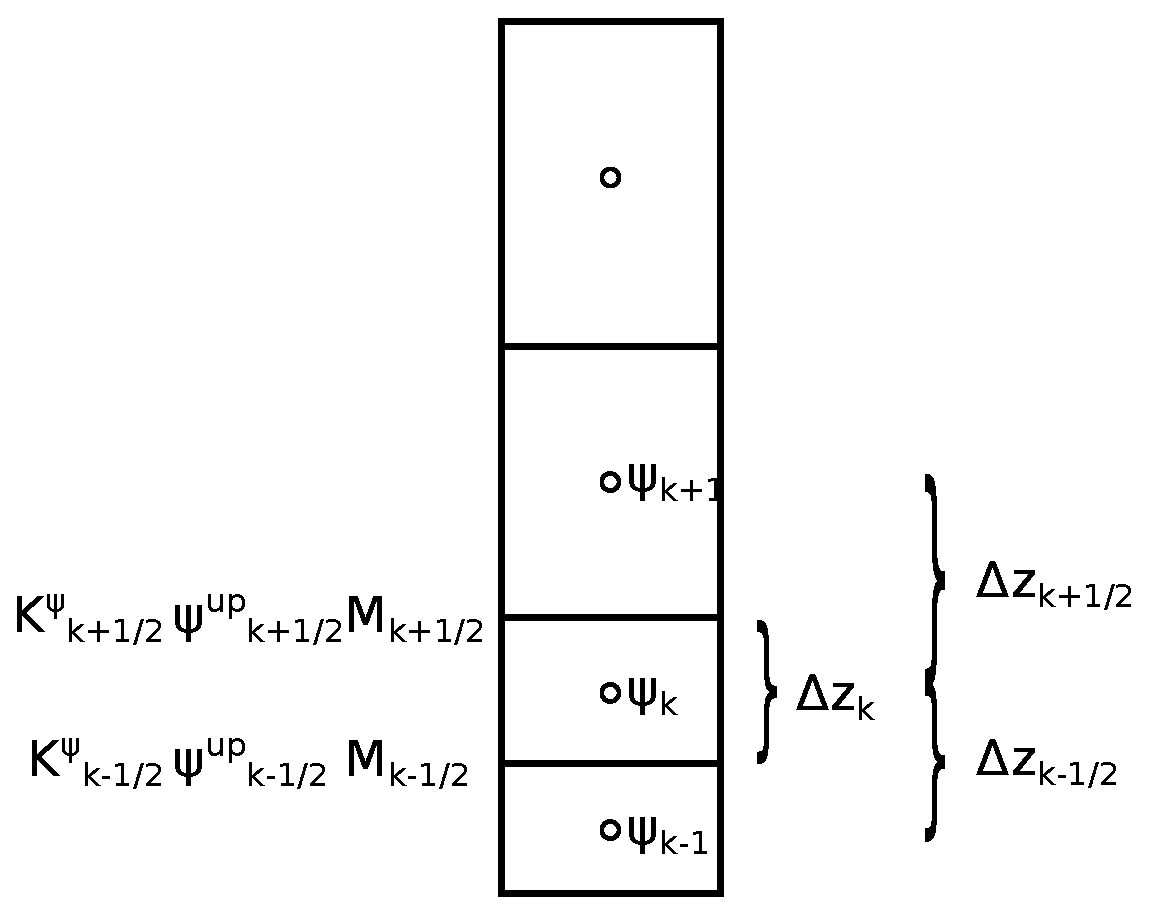
\includegraphics[width=0.5\textwidth]{staggering.eps}
\caption{Locations of prognostic variable $\psi$, the updraft mass fluxes $M_i$, the updraft properties $\psi^{up}_i$, and eddy-diffusivities $K^{\psi}$ on the 1D vertical grid. } \label{fig:staggering}
\end{figure}



\section{Cloud cover and interaction with radiation}\label{sec:clouds}

\subsection{Cumulus-topped PBL}

\subsection{Stratocumulus-topped PBL}



\section{Acknowledgements}
W.L. would like to thank Joao Teixeira and Kay Suselj for providing the code of their most recent version of the multiplume model. 


\bibliographystyle{ametsoc}
\input{documentation.bbl}
%\bibliography

 
\end{document}          

%\bibliography

 
\end{document}          

%\bibliography

 
\end{document}          


 
\end{document}          
